
\newcommand{\kpch}{\ensuremath{h^{-1} \, \text{kpc}}}
\newcommand{\kpc}{\ensuremath{\text{kpc}}}
\newcommand{\solarmh}{\ensuremath{h^{-1} \, M_\odot}}
\newcommand{\solarm}{M_\odot}
\chapter{Forming Vertical Structure in $\Lambda$CDM Discs}\label{ch:paper_iii}
\textbf{This chapter contains a draft of a paper submitted to Monthly Notices of the Royal Astronomical Society. Its current manuscript ID is MN-19-3241-MJ.}

\newpage
\section{Abstract}

We perform numerical experiments where stellar discs are inserted into
dark matter haloes in a $\Lambda$CDM simulation after which the
fully-live disc-halo systems are evolved until the present epoch. {Prior it its insertion, a disc is treated as a growing, rigid potential whose position and orientation are determined from rigid-body dynamics. When the disc goes live, the disc-halo system is in approximate equilibrium.} The
discs develop structures such as bars, warps, and bending waves.  Not
surprisingly, we find that when we insert the disc at a redshift
$z=1$, it develops more structure and exhibits more clearly signs of
disequilibrium then when it is inserted later.  We identify
populations of stars kicked out of the disc to high latitudes that are
qualitatively similar what is observed in the Milky Way. {An in-depth attempt is made to disentangle the effects of bar buckling, tidal fields due to 
the generally triaxial halo and from distant subhaloes, and the
passage of subhaloes through the inner disc. }While our
results are consistent with the hypothesis the the kicked-out-disc was
produced by a very massive satellite galaxy, we also find that they
can arise from the interaction of the disc with its halo. We conclude
that in the Milky Way a wide variety of cosmological environments are
able to explain disc structures like Monoceros, A13, and TriAnd.


%%%%%%%%%%%%%%%%%%%%%%%%%%%%%%%%%%%%%%%%%%%%%%%%%%

%%%%%%%%%%%%%%%%%%%% REFERENCES %%%%%%%%%%%%%%%%%%

% The best way to enter references is to use BibTeX:
\section{Introduction} \label{sec:introduction}

The \textsc{Hi} discs of late-type galaxies, when observed edge-on,
often exhibit pronounced warps (see, for example,
\citet{sancisi_1976,bosma_1991, garcia-ruiz_2002} and reviews by
\citet{binney_1992} and \citet{Sellwood2013}). Indeed, the \textsc{Hi}
warp in the Milky Way has been known since the work of
\citet{oort_1958}. There is also evidence for a stellar warp in the
Milky Way, which roughly traces that of the \textsc{Hi} disc
\citep{cox_1996, reyle_2009}.

The prevalence of warps suggests that a typical stellar disc
experiences perturbations normal to its midplane. Recent surveys,
particularly of the stellar content in the Galaxy, have revealed other
manifestations of vertical perturbations. For example, surveys such as
the Sloan Extension for Galactic Understanding and Exploration (SEGUE)
and Gaia Data Release 2 (GDR2) have uncovered an asymmetry with
respect to the Galactic midplane in stellar number counts in the
vicinity of the Sun \citep{widrow_2012_sdss, yanny_gardner_2013,
  bennet_2019_gaia}. In addition, bulk motions of stars normal to the
midplane have been found in data from SEGUE, the Radial Velocity
Experiment (RAVE), the LAMOST survey, and GDR2
\citep{widrow_2012_sdss, williams_2013_rave, carlin_2013_lamost,
  pearl_2017, carrillo_2018_rave, gaia_collab}. Furthermore, a
corrugation in stellar number counts with a wavelength of $\sim
5\,{\rm kpc}$ and an amplitude of $\sim 100\,{\rm pc}$ has been
detected between $10$ and $15$ kpc in Galactocentric radii
\citep{xu_2015}. Corrugations in the velocity field of gas discs
in external galaxies have also been observed \citep[for
  example]{matthews_2008,sanchez_2015}.

In addition to waves and corrugations, several stream-like stellar
structures in the Milky Way may have originated within the
disc. In the past, these structures were thought to comprise stars
tidally stripped from disrupted dwarf galaxies or globular
clusters. Recently, the idea that some of the streams are actually
stars 'kicked out' of the disc has gained traction. One example is the
Monoceros ring \citep{newberg_2002, yanny_2003}, also called the
Galactic Anticentre Stellar Structure (GASS) \citep{crane_2003,
  rocha-pinto_2003}, which is located at low latitudes towards the
Galactic anti-centre at a Galactocentric distance of about
$18\,\,\kpc$. The coincidence in position and velocity of GASS and
disc stars suggests that a disc origin may be a more likely explanation than tidal stripping \citep{deason_2018,
  monoceros_disk_origin}. Similar structures have been found in the
outer disc, most notably the Triangulum-Andromeda clouds (TriAnd)
\citep{triand_discovery} and A13 \citep{a13_discovery}. There is also
evidence for kicked-out stars in M31 \citep{richardson_2008_m31,
  dorman_2013_m31, bernard_2015_m31} and M33
\citep{mcconnachie_2006_m33, mcconnachie_2010_m33}. (For a review of
the kicked-out-disc hypothesis, see \citet{johnston_kud_review}.)

There is now a concerted effort to explain vertical disequilibria in
Milky Way-like galaxies. Much of this effort has focused on the
hypothesis that a single massive subhalo, such as the Sagittarius
dwarf spheroidal galaxy (Sgr dSph) \citep{ibata_discovery}, is
responsible for much of the vertical structure in the Milky
Way. Simulations of a single satellite encounter with an isolated
galaxy have been used to study this hypothesis \citep[for
  example]{purcell2011,gomez_2013,widrow_2014,feldmann_2015, dlv_2015,
  donghia_2016, laporte_2016, laporte_2018, laporte_2018_b}. While
many of the observed features are easily reproduced in the
simulations, it appears that a very massive ($10^{11}\,\solarm$) Sgr
dSph-like satellite is required to explain the extraplanar streams in
the outer disc \citep{laporte_2018_b}.

The single-satellite encounter is a rather idealized scenario;
disc-environment interactions in real galaxies will, of course, be
more complicated. In particular, discs may be continually perturbed by
any number of satellites or dark matter subhaloes whose orbits take
them into the disc region of the galaxy. Early steps toward a more
realistic model were taken by \citet{font_2001} and
\citet{gauthier_2006} who allowed for a system of subhaloes. In
particular, \citet{gauthier_2006} simulated an M31-like disc in a dark
halo where roughly 10\% of the smooth halo mass was replace by dark
subhaloes with a mass spectrum motivated by cosmological $\Lambda$CDM
simulations. They found that one or more of the subhaloes triggered the
formation of a bar. Further analyses of this simulation and a similar
one by \citet{chequers_2018} found that the system of subhaloes could
excite a plethora of vertical structure. However, these simulations
failed to create the streams of disc stars described above.

When a satellite passes through the plane of disc, it interacts with
the disc through a process akin to dynamical friction. Essentially,
disc stars fall in behind the satellite, disrupting and ultimately
heating the disc \citep{sellwood_1998}. On the other hand a distant
but very massive satellite can excite bending modes via differential
acceleration. In the simple example of a satellite falling toward the
disc along its spin axis, the acceleration of the disc toward the
satellite decreases with radius. Thus, as the satellite passes
through the centre of the disc, it will set up axisymmetric bending
modes as seen in \citet{sellwood_1996}.

Finally, we note that dark haloes in $\Lambda$CDM cosmologies are
thought to be aspherical and will therefore exert torques on the disc
that can cause it to bend and warp. The effect is due to a
misalignment of the disc symmetry axis with any of the approximate
symmetry axes of the halo. For example, \citet{hu_2016} embed discs
in triaxial haloes. In their appendix, strong warps can be seen in
discs which are substantially misaligned from their
haloes. \citet{gomez_2017} found that vertical structure was
ubiquitous in their hydrodynamical cosmological simulations, some of
which did not have discs in a stable orientation to their host halo.

In this paper, we study the vertical structure that develops in discs
embedded in realistic $\Lambda$CDM haloes. We use a disc insertion
scheme to set up initial conditions where a stellar disc is in
approximate equilibrium with a cosmological halo
\citep{berentzen_2006, debuhr_2012, ys_2015, bauer2018a, hu_2018}. Our
scheme affords us more control over the structural properties of the
disc than would be possible in fully self-consistent hydrodynamical
simulations and was successfully used to study bar formation in a
cosmological context in \citet{bauer2018b}. In fact, bar buckling is
another mechanism for exciting vertical structure in stellar discs
\citep{bar_buckling_echo}, a point we return to later in this paper.

Our paper is organized as follows: In \S\ref{sec:overview} we present
two toy models that serve to illustrate the mechanisms by which
satellites can excite bending modes in a stellar disc. An overview of
the cosmological simulations is given in \S\ref{sec:description} while
the time evolution and key structural features of the discs in these
simulations are discussed in \S \ref{sec:evolution}. In \S\ref{sec:kud}
we examine how stars are kicked out of discs.  We relate our key
results to other studies in \S\ref{sec:discussion} and present a
summary and some concluding remarks in \S\ref{sec:conclusion}.

\begin{figure}
	\centering
	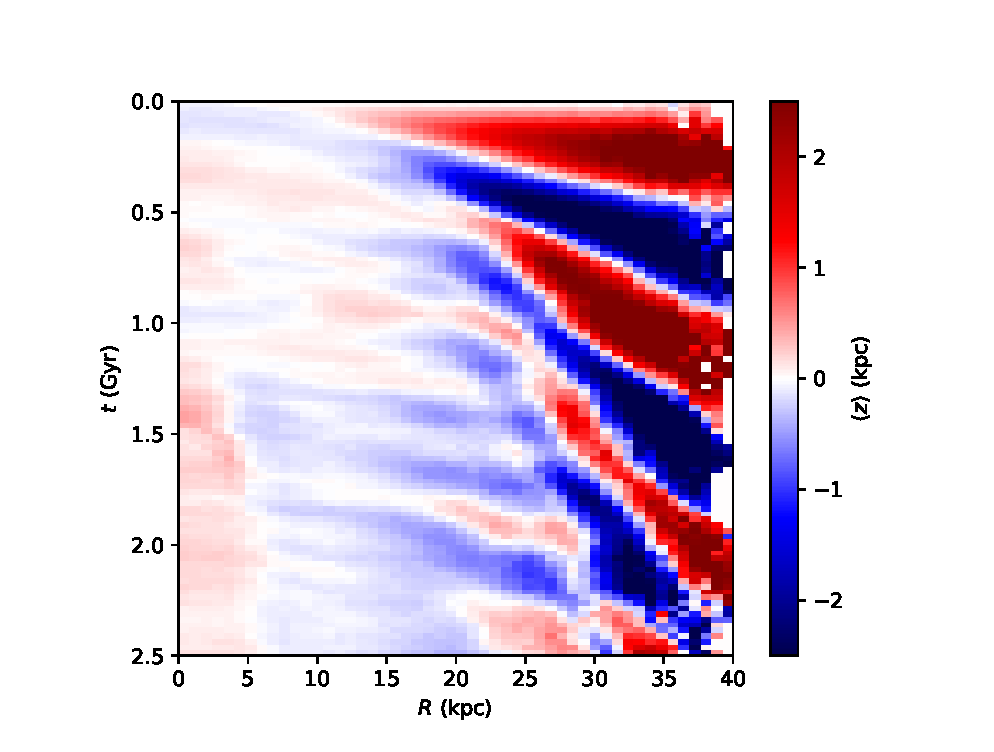
\includegraphics[width=0.85\textwidth]{../figures/isolated_z_0_r_a.eps}
	\caption{Mean vertical displacement, $\langle z \rangle$, of the disc for the
          toy model described in \S\ref{ssec:toy_model_1} as a
          function of $R$ and $t$.} \label{fig:toy_model_1_mean_height}
\end{figure}

\begin{figure}
	\centering
	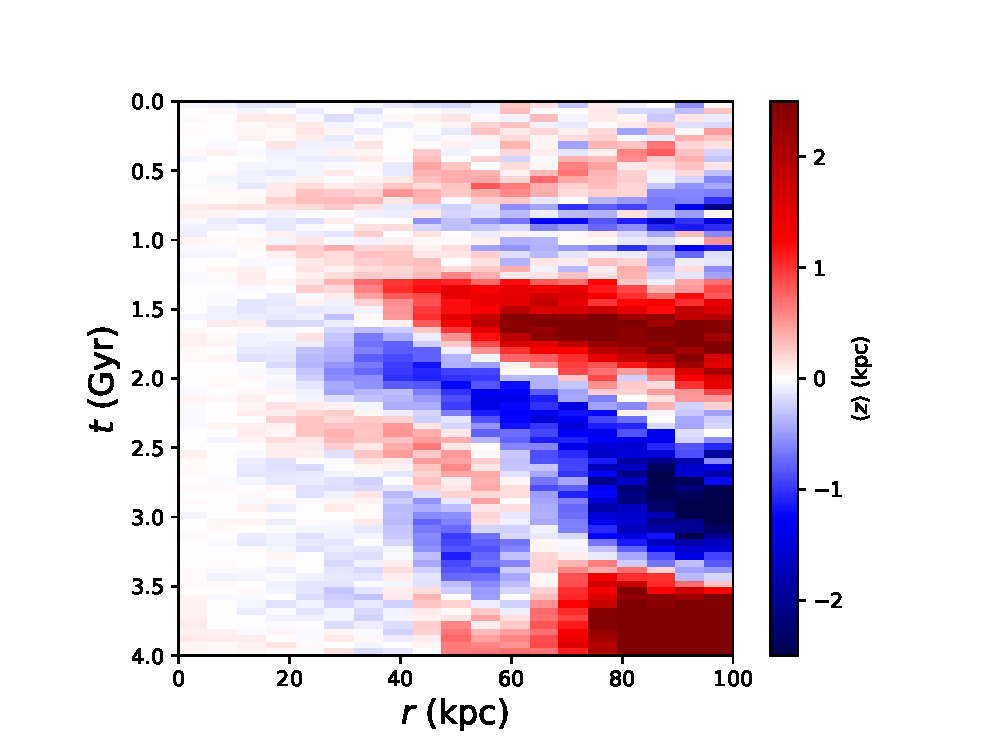
\includegraphics[width=0.85\textwidth]{../figures/isolated_z_0_r_a_halo.eps}
	\caption{Mean vertical displacement of the halo in the toy model described in
          \S\ref{ssec:toy_model_1} as a function of spherical radius $r$ and $t$.} 
        \label{fig:toy_model_1_mean_height_halo}
\end{figure}

\section{Single satellite simulations} \label{sec:overview}

In this section, we illustrate some of the factors driving vertical
structure in stellar discs through two toy models where a disc
interacts with a single subhalo.

\subsection{Axisymmetric subhalo encounter} 
\label{ssec:toy_model_1}

In our first experiment, the subhalo is initially at rest and
positioned $100\,{\rm kpc}$ from the centre of the disc along its
symmetry axis. We generate the initial conditions for the disc, halo,
and subhalo using the \textsc{GalactICS} code
\citep{KGGalactICSReference,WPDGalactICSReference}. The disc has an
exponential surface density with scale length $R_d=3.7\,\kpc$ and mass
$M_d=4\times10^{10} \,\solarm$. The halo has an NFW density profile
\citep{navarro_1997}, with scale length $R_h=33.2\,\kpc$, virial mass
$M_h=1.1\times10^{12}$, and concentration $c=6.7$. We use $10^6$ halo
particles and $3.5 \times 10^{6}$ disc particles. The subhalo is also
assumed to have an NFW profile with scale length $R_h=1.70\,\kpc$,
virial mass $M_h=2.7\times10^{10}$, and concentration $c=38.1$. The
choice of parameters for the disc, halo, and subhalo are motivated by
examples from our suite of cosmological simulations. The simulation is
performed using \textsc{Gadget-3}, a privately released version of the
popular \textsc{Gadget-2} code \citep{GadgetCodePaper}.

In Fig. \ref{fig:toy_model_1_mean_height} we show the azimuthally
averaged vertical displacement, $\langle z\rangle(R,\,t)$. The displacement
is relative to the disc midplane, defined by the mean $z$ of all the
particles. {
This quantifies axisymmetric vertical perturbations, that is, $m=0$
vertical perturbations where $m$ is the azimuthal mode number.  More generally, for a quantity $\Theta$, we define the $m$-fold symmetric $\Theta_m$,}
\begin{eqnarray}
\Theta_{m} &=&\frac{1}{M_S} \int_S \text{d}^3 \textbf{r} \text{d}^3\textbf{v} f(\textbf{r}, \textbf{v}) \Theta(\textbf{r} , \textbf{v})e^{i m \phi_j}\\
&\approx& \frac{1}{M_S} \sum_{j \in S} m_j \Theta(\textbf{r}_j, \textbf{v}_j)e^{im \phi_j} \label{eq:z_statistic}
\end{eqnarray}
{where $M_S$ is the mass in a region $S$, $f(\textbf{r},\textbf{v})$ is the phase space distribution function, $\phi_j$ is the azimuthal angle of the $j$-th particle in $S$, and $m_j$ is the mass of the $j$-th particle in $S$. 
}

At first the disc is relatively unperturbed; the subhalo is
so far away that it exerts an approximately uniform acceleration
across the disc. Only in the very outer disc do we see slight disc
flapping, that is, a lagging of the outer disc relative to the inner
one. The lag is more pronounce as the subhalo makes its first
pericentric passage. After the subhalo has passed through the disc, at
about $1\,{\rm Gyr}$, the pattern reverses as the center of the disc
is pulled back down. The resulting lag of the outer disc then shows up
as a positive signal. The disc develops a corrugation pattern as seen
in the alternating red and blue bands (positive and negative $\langle
z\rangle$). These bending waves propagate outward (bands stretch down
and to the right in the figure.) Over time, the wavelength decreases
as does the speed of propagation. Note that the strong ($> 1\,{\rm
  kpc}$) flapping of the disc beyond $20\,{\rm kpc}$ persists for many
dynamical times (see, also \citet{sellwood_1996}) and weaker
corrugation patters are seen further in.

Qualitatively similar behaviour is seen in the halo. In
Fig. \ref{fig:toy_model_1_mean_height_halo} we show $\langle
z\rangle$, this time averaged in spherical shells in the halo. At
early times, the halo is dragged along with the subhalo. Eventually,
we get a sloshing back and forth of the halo.

\begin{figure}
	\centering
        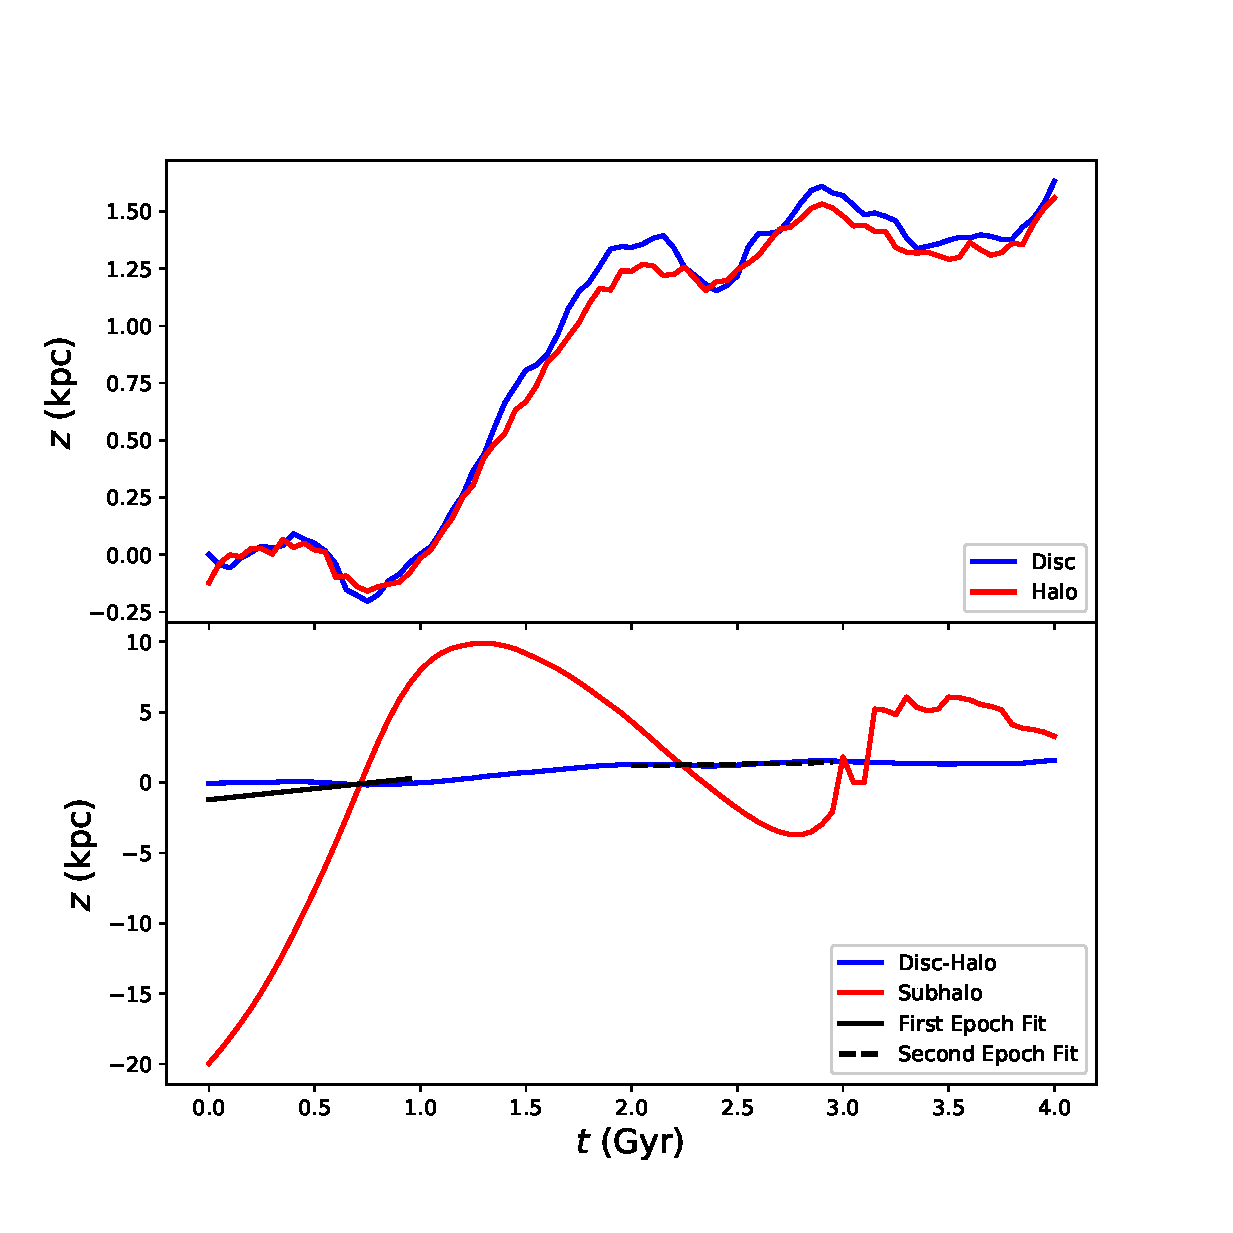
\includegraphics[width=0.85\textwidth]{../figures/isolated_orbits_two_fits_two_panel.eps}
	\caption{Top panel: Orbit of the disc (blue) and inner halo
          (red) in the toy model described in
          \S\ref{ssec:toy_model_2}. Only the $z$-components of the
          disc and halo position vectors are shown. Bottom panel:
          Orbits of the disc and inner halo (blue) and subhalo
          density peak (red).  The black lines show the fits for the
          two epoch as described in the
          text.} \label{fig:toy_model_2_orbits}
\end{figure}

\subsection{Off-axis subhalo encounter} \label{ssec:toy_model_2}
\begin{figure}
	\centering
	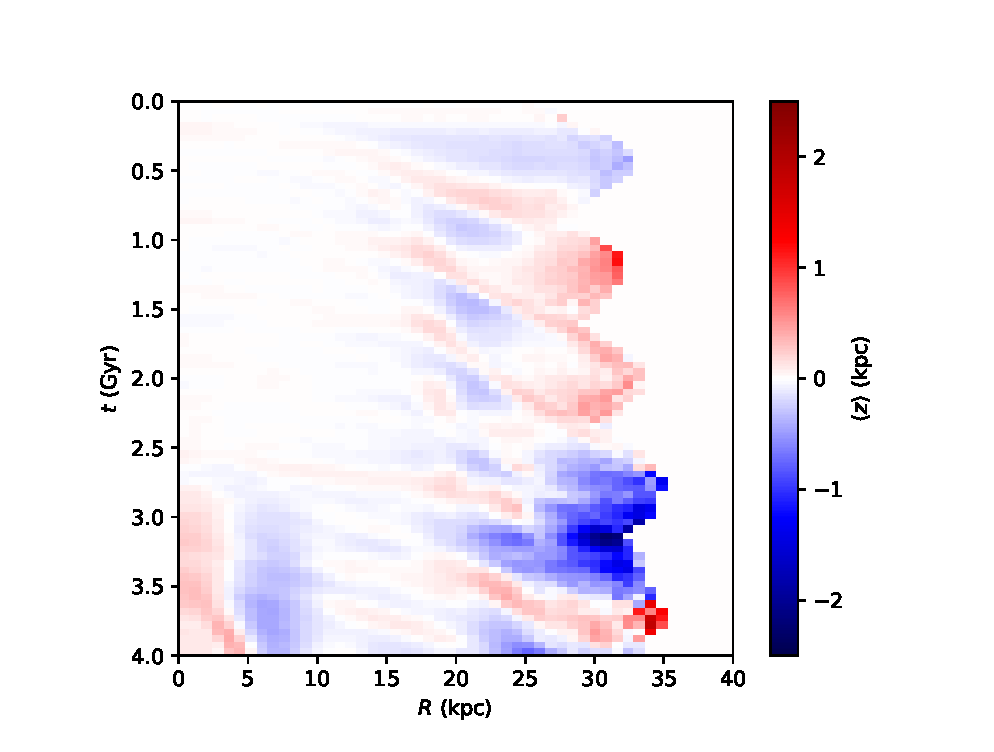
\includegraphics[width=0.85\textwidth]{../figures/b_late_light_subhalo_z_0_r_a.eps}
	\caption{Mean height, $\langle z \rangle$, of the disc for the
          toy model described in \S\ref{ssec:toy_model_2} as a
          function of $R$ and
          $t$.} \label{fig:toy_model_2_mean_height}
\end{figure}

In our second experiment, the satellite is again initialized at rest
$100\,{\rm kpc}$ from the centre of the disc, but this time at an
angle of just $12^\circ$ from the disc plane. The choice of orbit is
motivated by a satellite in one of our cosmological simulations. The
parameters for the disc, halo, and subhalo are the same as in
\S\ref{ssec:toy_model_1}.

In the upper panel of Fig. \ref{fig:toy_model_2_orbits} we plot the
$z$ coordinates of the position vector ${\bf r}_d$ of the disc and
${\bf r}_h$, the position vector of the peak halo density.  Evidently,
the halo density peak and centre of the disc closely track one
another. We next define a common position vector for the disc and
inner halo:
\begin{equation}
{\bf r}_{dh} = \frac{M_d {\bf r}_d + M_{h,20} {\bf r}_{h,20}}
{M_d + M_{h,20}}
\end{equation}
\noindent where we have arbitrarily used $20\,{\rm kpc}$ to define the
inner halo. Given the closeness of ${\bf r}_d$ and ${\bf r}_h$, the
choice of this definition shouldn't effect the results that follow.

Our working hypothesis is that during periods between perigalactic passages,
the subhalo and the combination of the disc and inner halo can be
treated as a two-body system. That is, ${\bf r}_{dh}$ and ${\bf
  r}_{sh}$, where the latter is the position vector for the peak of
the subhalo, satisfy the equation
\begin{equation}
\frac{M_{dh}\textbf{r}_{dh} + M_{sh} \textbf{r}_{sh}}{M_{dh} +
  M_{sh}} = \textbf{r}_{c,0} + \textbf{v}_{c,0} t
\end{equation}
where $M_{dh}$ and $M_{sh}$ are the effective disc-halo and subhalo masses.

To test our hypothesis, we maximize the likelihood function
\begin{equation}
\ln \mathcal{L} = -\frac{\chi^2}{2\sigma_d^2} - N\ln\sigma_d / \kpc
\end{equation}
over the parameters ${\bf r}_{c,0}$, ${\bf v}_{c,0}$, $M_{dh}$,
and $M_{sh}$. Here, $N$ is the number of snapshots, {$\sigma_d$ is the RMS difference between the model and the data, }and
\begin{equation}
\chi^2 = \left\vert
\frac{M_{dh}\textbf{r}_{dh} + M_{sh} \textbf{r}_{sh}}{M_{dh} + M_{sh}}
- (\textbf{r}_{c,0} + \textbf{v}_{c,0} t )\right\vert^2~.
\end{equation}
Maximization is done in two $1 \, {\rm Gyr}$  epochs centered on $0.5\,{\rm
  Gyr}$ and $2\,{\rm Gyr}$, respectively. These windows are chosen to
avoid the pericentric passages at $0.85\,{\rm Gyr}$ and $3\,{\rm
  Gyr}$, when the subhalo is losing the most mass when the system will
be poorly described by a two-body model. The center-of-mass motion
lines, $\textbf{r}_{c,0} + \textbf{v}_{c,0} t$ for the two epochs are
shown in Fig. \ref{fig:toy_model_2_orbits}. The inferred effective
mass ratios $M_{sh}:M_{dh}$ are 16:1 and 85:1, respectively.  Thus,
the effective mass of the subhalo has been reduced by a factor of
$\sim 5$, presumably due to tidal stripping. We also find that
$\sigma_d= 190\,{\rm pc}$ and $290\,{\rm pc}$ for the two epochs.  The
fact that the values for $\sigma_d$ are as small as they are supports
our hypothesis of a two-body model for the disc-halo/subhalo system.

In Fig. \ref{fig:toy_model_2_mean_height} we plot the mean height
across the disc as a function of radius and time. The general
corrugation pattern is similar to the one seen in our first experiment
though the amplitude is smaller. The difference in amplitude is no doubt
due to the fact that we are averaging over azimuth in an experiment
that lacks azimuthal symmetry.

\section{Simulations} \label{sec:description}

In this section, we summarize our cosmological simulations beginning
with a brief description of our disc insertion scheme.

\begin{figure}
	\centering
	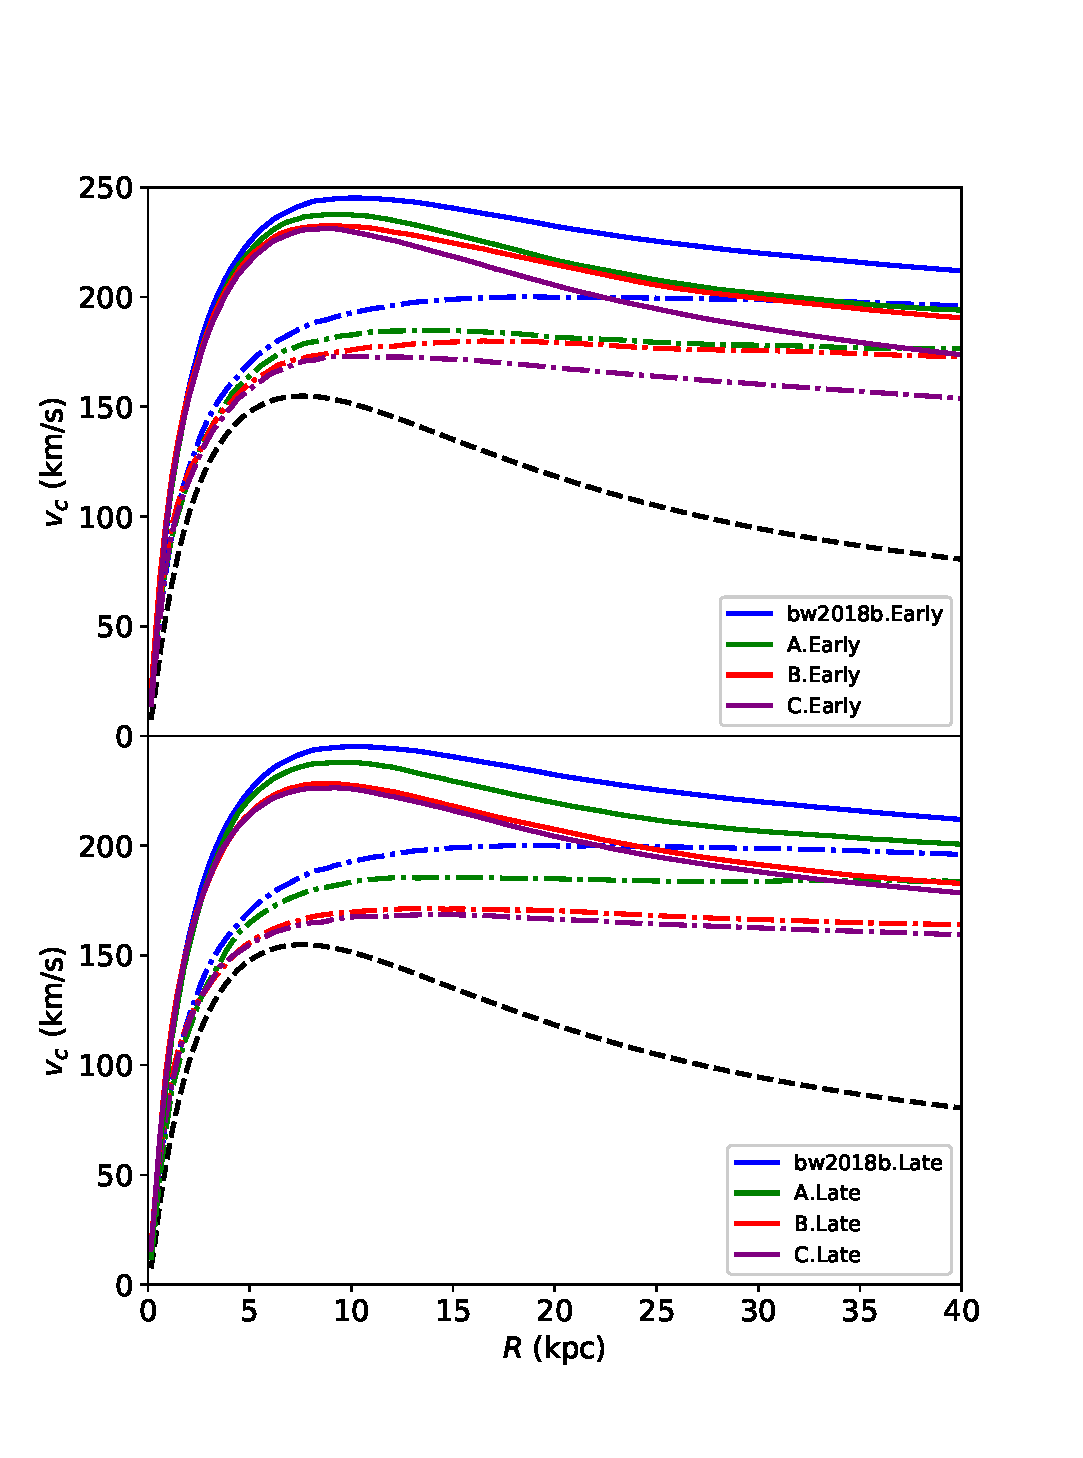
\includegraphics[width=0.85\textwidth]{../figures/rotation_curve.eps}
	\caption{Circular speed curves for cosmological models. The
          same disc is used in all runs, and its rotation curve
          contribution is shown by the black dashed line. The halo
          contributions for the Early and Warm subsuites are shown in
          the top panel as dot-dashed lines, while the total rotation
          curves are shown as solid curves. The bottom panel shows the
          same for the Late subsuite.} \label{fig:rotation_curves_iii}
\end{figure}

\begin{figure}
	\centering
	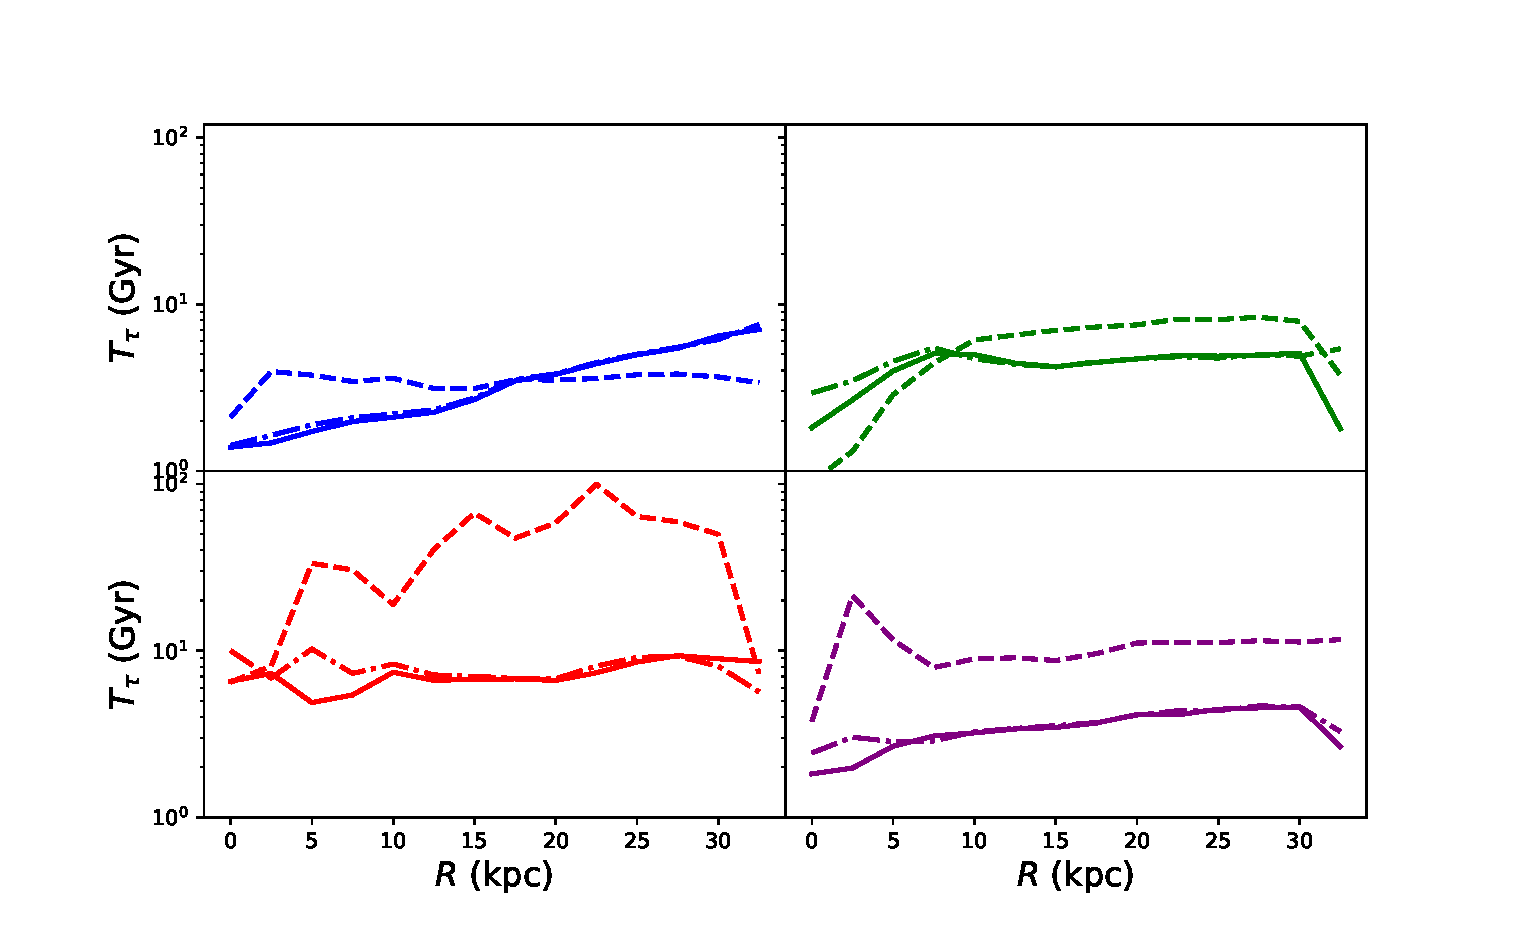
\includegraphics[width=0.85\textwidth]{../figures/timescale.eps}\caption{The
          torque timescale, $T_\tau$, at initialization as a function of $R$.
          Colours are the same as in
          Fig. 5 with bauer2018b in the upper left panel, A in the upper right,
          B in the lower left, and C in the lower right.
          Line types are Early (solid), Warm (dot-dashed), and
          Late (dashed).} \label{fig:ratio_freqs}
\end{figure}

\begin{figure}
	%\centering
	\hspace{-0.75in}
	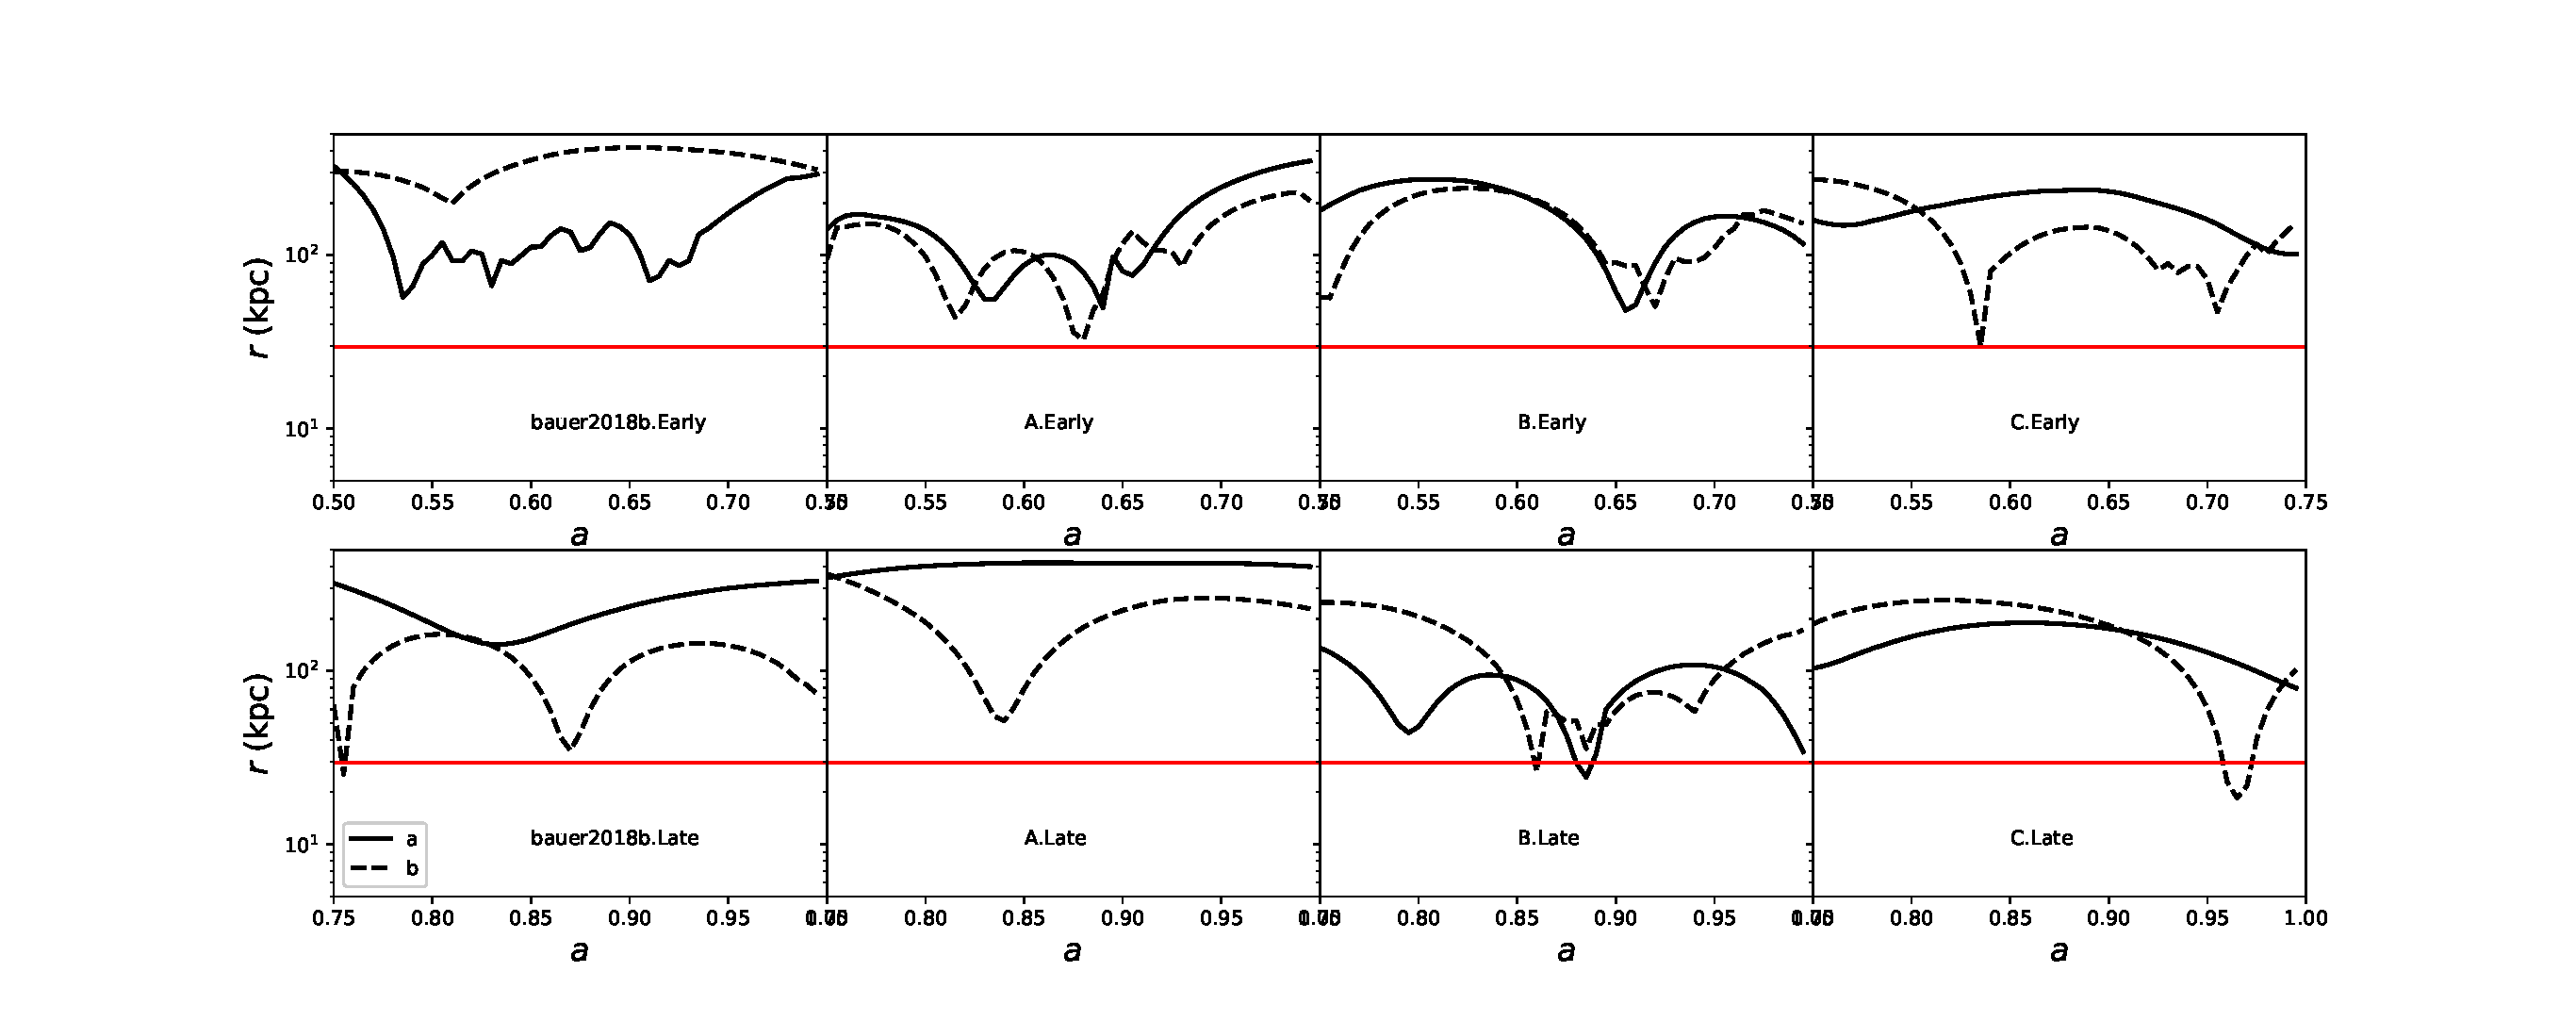
\includegraphics[width=1.2\textwidth]{../figures/substructure_r_vs_t.eps}
	\caption{Orbits of the most massive subhalo (solid curve)
          and second most massive subhalo (dashed curve) for the
          fiducial suite (top panel) and late insertion suite
          (bottom). These are the substructures listed as the top two
          entries for each simulation in Table
          \ref{tab:substructure}. The red line denotes $20\, \kpch =
          29.5 \, \kpc$. } \label{fig:substructure_orbits}
\end{figure}

\subsection{Disc Insertion Technique} \label{ssec:disc_insertio}

Our disc insertion scheme \citep{bauer2018a} expands upon the method
introduced by \citet{BerentzenShlosmanStellarDisks},
\citet{debuhr_2012}, and \citet{ys_2015}. It uses an iterative
procedure to initialize an axisymmetric, smooth disc in a cosmological
halo, that is generally clumpy and triaxial. The first step is to run
a pure dark matter simulation and identify a suitable halo. We then
rerun the simulation with a rigid disc potential that grows from zero
to that of the fully formed disc between an initial scale factor,
$a_g$, to a final scale factor, $a_l$.  When the simulation reaches
$a_l$, the rigid disc is replaced by an N-body system and the ``live''
disc-halo system is evolved to the present epoch at $a=1$.

For our pure dark matter simulation, we implement the zoom-in
technique of \citet{KatzQuasarZoom} and \citet{NavarroWhiteZoom}.  We
select Milky Way-like haloes with no major mergers and use the results
of \cite{onorbe_etal_2014} to ensure minimal contamination of
low-resolution particles.  Our choice of cosmological parameters is
based on the results from Planck 2013 \citep{planck_2014}:
$H_0=67.9\,{\rm km\,s}^{-1}\,{\rm kpc}^{-1}$, $\Omega_b = 0.0481$,
$\Omega_0 = 0.306$, $\Omega_\Lambda = 0.694$, $\sigma_8 = 0.827$, and
$n_s = 0.962$. N-body initial conditions for the dark matter particles
are generated with the \textsc{music} code \citep{music}.

During its growth phase from $a_g=0.25$ to $a_l=0.5$\footnote{For
  reference, $a=0.25$ is 2.2 Gyr after the Big Bang, $a=0.5$ is 5.9
  Gyr after the Big Bang, and $a=0.75$ is 10.0 Gyr after the Big
  Bang. The age of this Universe at present day is 13.8 Gyr.}, the
disc is treated as a rigid body whose orientation and center-of-mass
position evolve according to the standard equations of rigid body
dynamics. \citet{bauer2018a} found that the rigid disc assumption is
actually quite true to the orientation and center of mass evolution of
a pure stellar disc. At $a_l$, we swap a live disc for the rigid one
using a modified version of \textsc{GalactICS}
\citep{KGGalactICSReference,WPDGalactICSReference}, which generates a
three-integral DF disc in the best axisymmetric approximation to the
halo \citet{bauer2018a}.

\subsection{Numerical Experiments} \label{ssec:numerical_experiments}

We present a concise description of our cosmological models in Table
\ref{tab:sims_iii}. The haloes are chosen such that the total circular
speed curves are similar to the Milky Way's. Note that the bauer2018b
simulations use a halo from \cite{bauer2018b}. The haloes used in the
A, B, and C simulations are previously unpublished.  In the
simulations denoted as X.Early, the disc is inserted at $a_l=0.5$; for
those denoted X.Lake, $a_l=0.75$.  One of the benefits of disc
insertion techniques is the ability to modify disc properties in the
same halo. We exploit this capability in our third suite, denoted as
X.Warm, where we increase the disc's dynamical temperature as
measured by the Toomre $Q$ parameter \citep{toomre_q}.
 
Fig. \ref{fig:rotation_curves_iii} shows the circular speed curves for all
disc-halo combinations. There are relatively small variations in the
circular speed for $R<5\,{\rm kpc}$ where the disc dominates. The
variations are significant ($\sim 10\,{\rm km\,s}^{-1}$) near the peak
of the circular speed curve and even larger beyond the disc where the
halo dominates the gravitational potential. In all cases, the disc is
submaximal. In particular, the ratio of the square of the disc
contribution to the rotation curve and square of the total rotation
curve measured at $2.2\, R_d$, $\left. V_d^2/V_{tot}^2 \right
\vert_{R=2.2\,R_d}$, ranges between 0.37 and 0.46. These values are
well below the lower bound for a maximal disc advocated by
\citet{sackett_1997}.

In the discussion that follow, we focus on three archetypal
simulations:
\begin{enumerate}
\item \textbf{strong disc-subhalo interaction:} In B.Late the disc has close
  interactions with two subhaloes but no substantial disc-halo
  misalignment. One of these subhaloes passes twice through the plane
  of the disc.
\item \textbf{disc-halo misalignment:} C.Early presents a case a
  substantial misalignment from its host halo (see below) but
  relatively modest subhalo interactions with the disc.
\item \textbf{distant massive subhaloes:} The disc in A.Early is relatively
  well aligned to its host halo, but its most massive substructures do not
  interact closely with the disc.
\end{enumerate}

To illustrate how the simulations differ, consider
Fig.\,\ref{fig:torque} where we plot the component of the torque
perpendicular to the spin axis of the disc across the disc plane. In
B.late, we have the localized effect of a subhalo that passes through
the plane of the disc. On the other hand, in C.Early, we have a strong
$m=2$ torque due to the large-scale structure of the halo and
misalignment of the disc with any of the halo's approximate symmetry
axes.

\begin{figure}
	\centering
	\subfloat[]{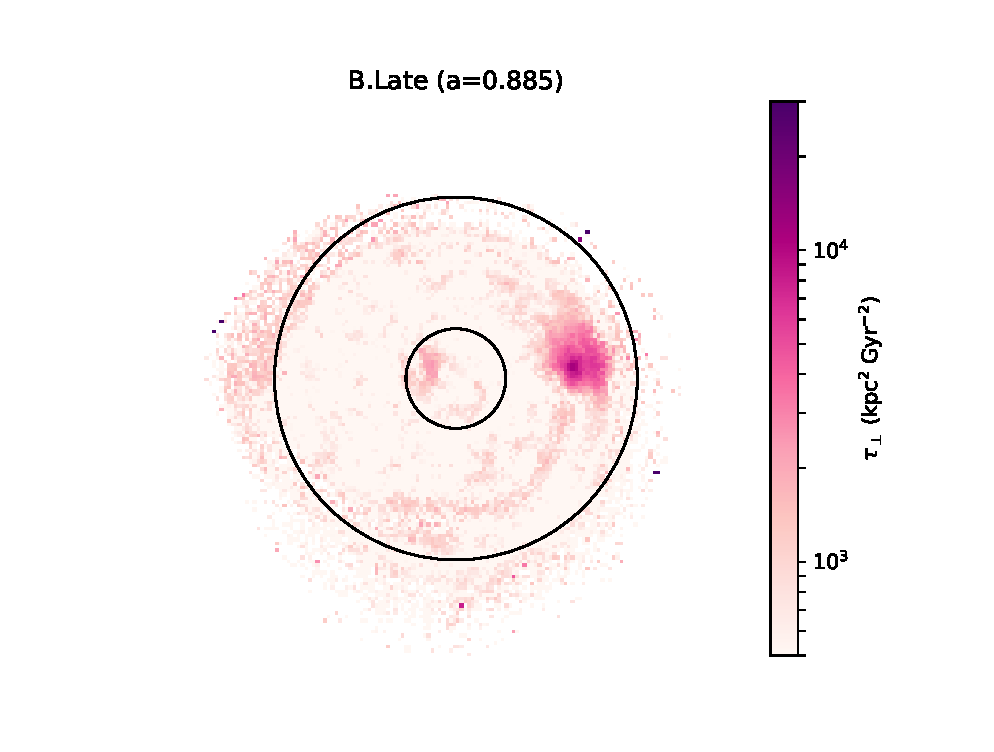
\includegraphics[width=0.8\textwidth]{../figures/b_late_torque_a_0_885.eps}}\\
	\subfloat[]{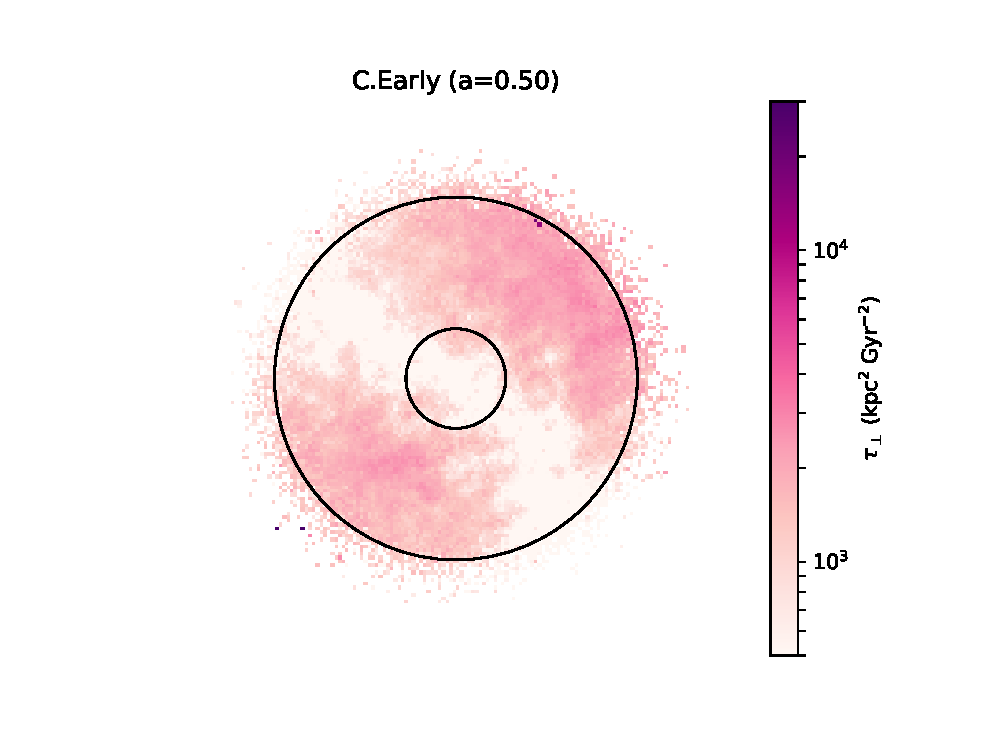
\includegraphics[width=0.8\textwidth]{../figures/c_early_torque_a_0_5.eps}}
	\caption{The component of the torque perpendicular to the spin
          axis of the disc across the disc plane. Top
          panel is for B.Late at $a=0.885$ when the most massive
          subhalo is at pericentre.  The bottom panel is for C.Early
          at initialization ($a=0.5$). The circles correspond to $R_p
          = 2.2\,R_d=8.1\,\kpc$ and
          $20\,\kpch=29.5\,\kpc$.}\label{fig:torque}
\end{figure}

\begin{sidewaystable}
\centering
\caption{Table of simulations run in the main experiment. $M_h$ is the
  virial mass of the host halo, $R_h$ is the NFW scale length of the
  host halo, $c$ is the NFW concentration parameter of the host halo,
  $a_l$ is the live disc insertion scale factor, $\delta
  \Theta_{h,20}$ is the halo misalignment angle for the 20 kpc shell,
  $N_d$ is the number of disc particles, $Q$ is the Toomre stability
  parameter of the disc at initialization, and $f_{kud}$ is the
  fraction of disc mass that gets classified as kicked-out-disc (KOD)
  stars measured at present day with $\eta=8$.} \label{tab:sims_iii}
\begin{tabular}{l l l l l l l l l l}
\hline
       & $M_h\,\,(\solarm)$ & $R_h\,\,(\kpc)$ & $c$ & $a_l$ &  $N_d$ & $Q$ & $\cos\delta \Theta_{h,20}$ & $f_{kud}$\\
\hline
bauer2018.Early   & $1.0 \times 10^{12}$ & 15.9 &  9.84 &   0.50 & $1.0 \times 10^6$ & 1.1 & 0.16 & $1.2 \times 10^{-2}$\\
bauer2018.Warm    & $1.0 \times 10^{12}$ & 15.9 &  9.84 &   0.50 & $1.0 \times 10^6$ & 1.1 & 0.16 & $1.1 \times 10^{-2}$\\
bauer2018.Late    & $1.2 \times 10^{12}$ & 15.2 &  15.4 &   0.75 & $1.0 \times 10^6$ & 1.8 & 0.93 &$4.2 \times 10^{-3}$\\
A.Early           & $9.4 \times 10^{11}$ & 17.8 &  8.56 &   0.50 & $3.5 \times 10^6$ & 1.3 & 0.97 &$3.7 \times 10^{-3}$\\
A.Warm            & $9.4 \times 10^{11}$ & 17.8 &  8.56 &   0.50 & $3.5 \times 10^6$ & 1.8 & 0.97 & $1.6 \times 10^{-3}$\\
A.Late            & $1.1 \times 10^{12}$ & 18.5 &  12.1 &   0.75 & $3.5 \times 10^6$ & 1.3 & 0.98 & $6.8 \times 10^{-5}$\\
B.Early           & $5.9 \times 10^{11}$ & 10.4 &  12.6 &   0.50 & $3.5 \times 10^6$ & 1.3 & 0.91 & $8.5 \times 10^{-4}$\\
B.Warm            & $5.9 \times 10^{11}$ & 10.4 &  12.6 &   0.50 & $3.5 \times 10^6$ & 1.8 & 0.91 & $1.2 \times 10^{-3}$\\
B.Late            & $1.1 \times 10^{12}$ & 33.2 &  6.70 &   0.75 & $3.5 \times 10^6$ & 1.3 & 0.99 & $9.2 \times 10^{-4}$\\
C.Early           & $4.3 \times 10^{11}$ & 8.33 &  14.1 &   0.50 & $3.5 \times 10^6$ & 1.3 & 0.84 & $5.3 \times 10^{-3}$\\
C.Warm            & $4.3 \times 10^{11}$ & 8.33 &  14.1 &   0.50 & $3.5 \times 10^6$ & 1.8 & 0.84 & $5.6 \times 10^{-3}$\\
C.Late            & $6.7 \times 10^{11}$ & 13.6 &  14.0 &   0.75 & $3.5 \times 10^6$ & 1.3 & 0.92 & $1.0 \times 10^{-4}$\\
\hline
\end{tabular} 

\end{sidewaystable}

\subsection{Halo Environments} \label{ssec:halo_env}

To further quantify the effect of the halo environment we define a
torque timescale:
\begin{equation}
T_\tau(R) = \frac{L(R)}{\tau_\perp(R)},
\end{equation}
where $L(R)$ is the magnitude of the angular momentum in a ring
centered at radius $R$ and $\tau_\perp(R)$ is the azimuthally-averaged
component of the torque that is perpendicular to the spin axis of the
disc.  The greater the misalignment between disc and halo, the larger
the torque of the halo on the disc, and the shorter the timescale
$T_\tau$. In Fig. \ref{fig:ratio_freqs}, we plot $T_\tau$ as a
function of radius at initialization for our models. In general, the
effect of tidal torques from the halo are smaller at late times when
much of the substructure and triaxiality of the halo has been washed
out. We also infer that the effect of the halo in torquing the disc is
largest in C.Early.

In Table \ref{tab:substructure}, we list the five most massive (at
initialization) substructures for each of our simulations while the
orbits of the two most massive substructures are shown in
Fig. \ref{fig:substructure_orbits}.  The orbits present a wide variety
of behaviour. For example, the subhaloes in bauer2018b.Early spend
most of their lives in the outer halo on roughly tangential orbits. By
contrast, the second most mass subhalo in C.late orbits to within
$\sim 20\,{\rm kpc}$ of the disc centre. The subhaloes in A.early are
more massive but never reach to within $30\,{\rm kpc}$.

\begin{sidewaystable}
\caption{Table of the five most massive substructures at $a_l$ in all
  of the simulations detailed in Table \ref{tab:sims_iii}. The virial
  mass, $M_s$, and NFW scale radius, $R_s$, are
  given.}\label{tab:substructure}
	\begin{tabular}{|l l l l | l l l l|}
	\hline
	Subhalo Name ($z=1$) & $M_s \,(\solarm)$ & $R_s \, (\kpc)$ & $c$ & Subhalo Name ($z=0.333$) & $M_s \,(\solarm)$ & $R_s \, (\kpc)$ & $c$\\	
	\hline
    bauer2018b.Early.a & $1.4 \times 10^{10}$ & 3.75 & 9.92 & bauer2018b.Late.a & $1.6 \times 10^{10}$ & 3.35 & 16.5 \\
    bauer2018b.Early.b & $1.0 \times 10^{10}$ & 1.02 & 32.8 & bauer2018b.Late.e & $0.7 \times 10^{10}$ & 0.27 & 154. \\
    bauer2018b.Early.c & $0.5 \times 10^{10}$ & 2.60 & 10.1 & bauer2018b.Late.c & $0.3 \times 10^{10}$ & 0.07 & 485. \\
    bauer2018b.Early.d & $0.4 \times 10^{10}$ & 1.51 & 15.7 & bauer2018b.Late.d & $0.3 \times 10^{10}$ & 1.06 & 29.8 \\
    bauer2018b.Early.e & $0.2 \times 10^{10}$ & 0.28 & 69.0 & bauer2018b.Late.e & $0.2 \times 10^{10}$ & 0.38 &  76.7\\
	\hline
	A.Early.a & $1.8 \times 10^{10}$ & 2.69 & 15.3 & A.Late.a & $1.3 \times 10^{10}$ & 2.62 & 19.6 \\
	A.Early.b & $1.2 \times 10^{10}$ & 1.26 & 28.4 & A.Late.b & $0.9 \times 10^{10}$ & 0.61 & 74.8 \\
	A.Early.c & $1.0 \times 10^{10}$ & 0.71 & 47.9 & A.Late.c & $0.5 \times 10^{10}$ & 0.77 & 46.4 \\
	A.Early.d & $0.7 \times 10^{10}$ & 2.29 & 13.0 & A.Late.d & $0.4 \times 10^{10}$ & 1.69 & 19.7 \\
	A.Early.e & $0.5 \times 10^{10}$ & 1.73 & 13.2 & A.Late.e & $0.2 \times 10^{10}$ & 1.25 & 21.5 \\
	\hline
	B.Early.a & $1.1 \times 10^{10}$ & 1.76 & 19.4 & B.Late.a & $2.7 \times 10^{10}$ & 1.70 & 38.1 \\
	B.Early.b & $0.2 \times 10^{10}$ & 0.41 & 47.5 & B.Late.b & $1.2 \times 10^{10}$ & 2.27 & 22.0 \\
	B.Early.c & $0.2 \times 10^{10}$ & 0.67 & 28.4 & B.Late.c & $0.6 \times 10^{10}$ & 2.67 & 14.4 \\
	B.Early.d & $0.2 \times 10^{10}$ & 1.81 & 10.3 & B.Late.d & $0.4 \times 10^{10}$ & 1.42 & 24.0 \\
	B.Early.e & $0.2 \times 10^{10}$ & 0.54 & 34.0 & B.Late.e & $0.4 \times 10^{10}$ & 1.13 & 29.7 \\
	\hline
    C.Early.a & $1.0 \times 10^{10}$ & 1.78 & 18.5 & C.Late.a & $0.5 \times 10^{10}$ & 0.18 & 194. \\
	C.Early.b & $0.6 \times 10^{10}$ & 0.92 & 30.0 & C.Late.b & $0.4 \times 10^{10}$ & 6.37 & 5.46 \\
	C.Early.c & $0.3 \times 10^{10}$ & 2.24 & 10.2 & C.Late.c & $0.4 \times 10^{10}$ & 0.75 & 46.2 \\
	C.Early.d & $0.1 \times 10^{10}$ & 0.91 & 18.7 & C.Late.d & $0.3 \times 10^{10}$ & 1.26 & 26.1 \\
	C.Early.e & $0.1 \times 10^{10}$ & 0.25 & 60.3 & C.Late.e & $0.3 \times 10^{10}$ & 6.78 & 4.81 \\
	\hline
	\end{tabular}
\end{sidewaystable}

\section{Structure and Evolution of Simulation Models} \label{sec:evolution}

In this section we summarize the evolution of the models in our
simulations.  We begin with a discussion of bar formation and then
turn to bending and warping of the discs.

\subsection{Bar Formation}

\begin{figure}
    \centering
    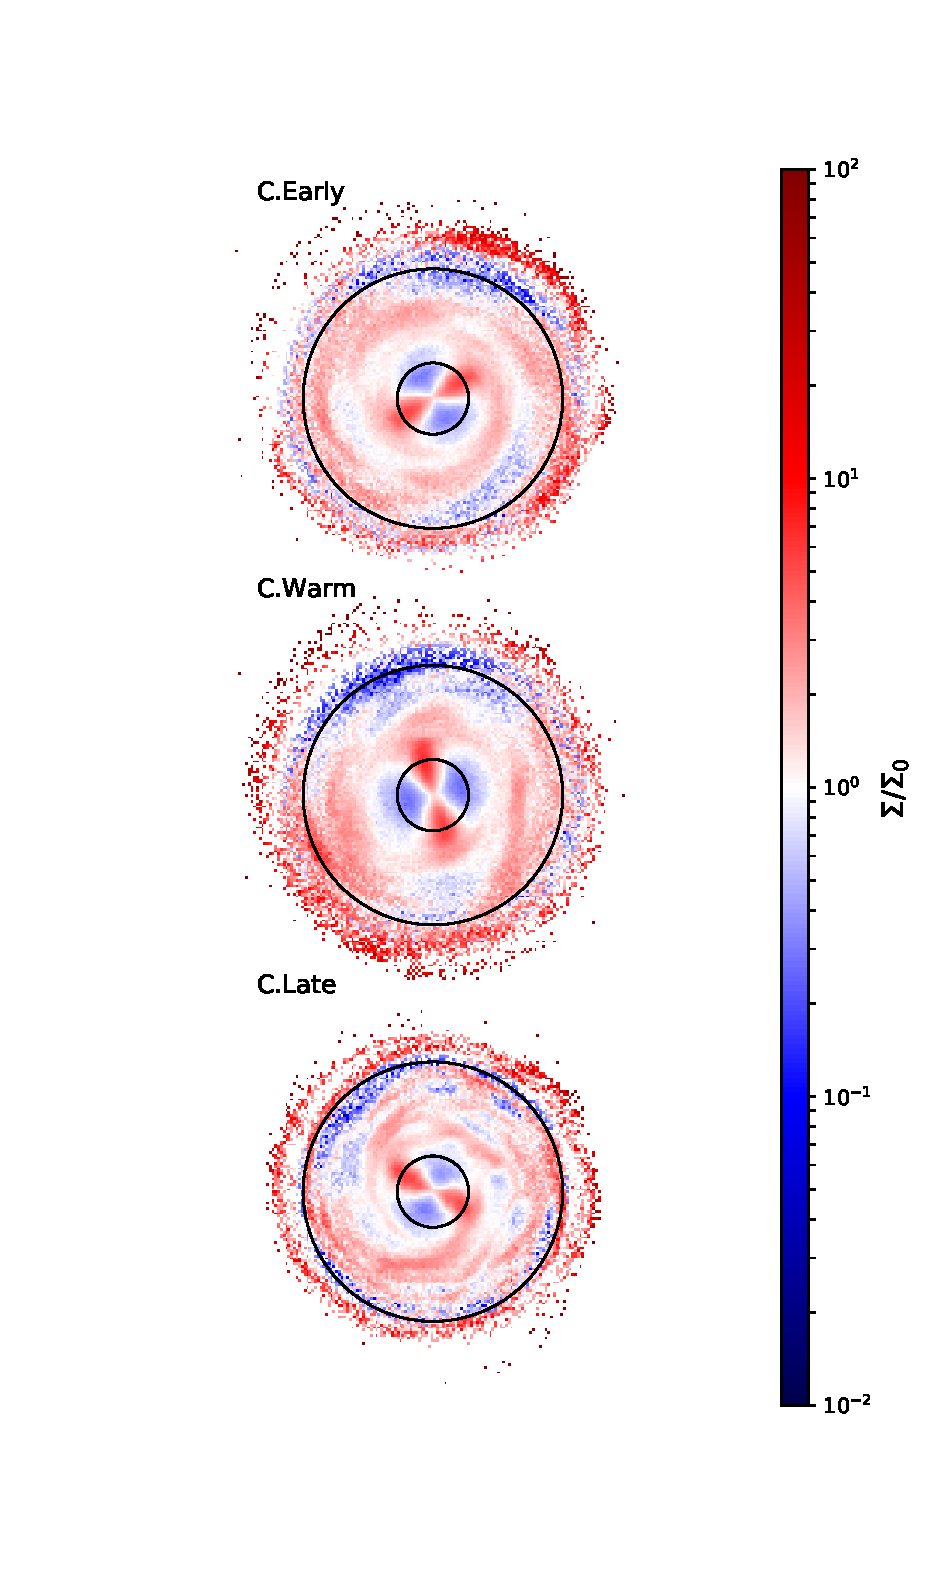
\includegraphics[width=0.7\textwidth]{../figures/surface_density_ratios.eps} \caption{The
      ratio of surface density, $\Sigma$, to azimuthally averaged
      surface density, $\Sigma_0$ for the C.Early, C.Warm, and C.Late
      models. The circles correspond to $R_p = 2.2\, R_d = 8.1 \,\kpc$
      and $20 \,\kpch = 29.5 \, \kpc$.}
	\label{fig:final_densities}
\end{figure}

\begin{figure}
	\centering
	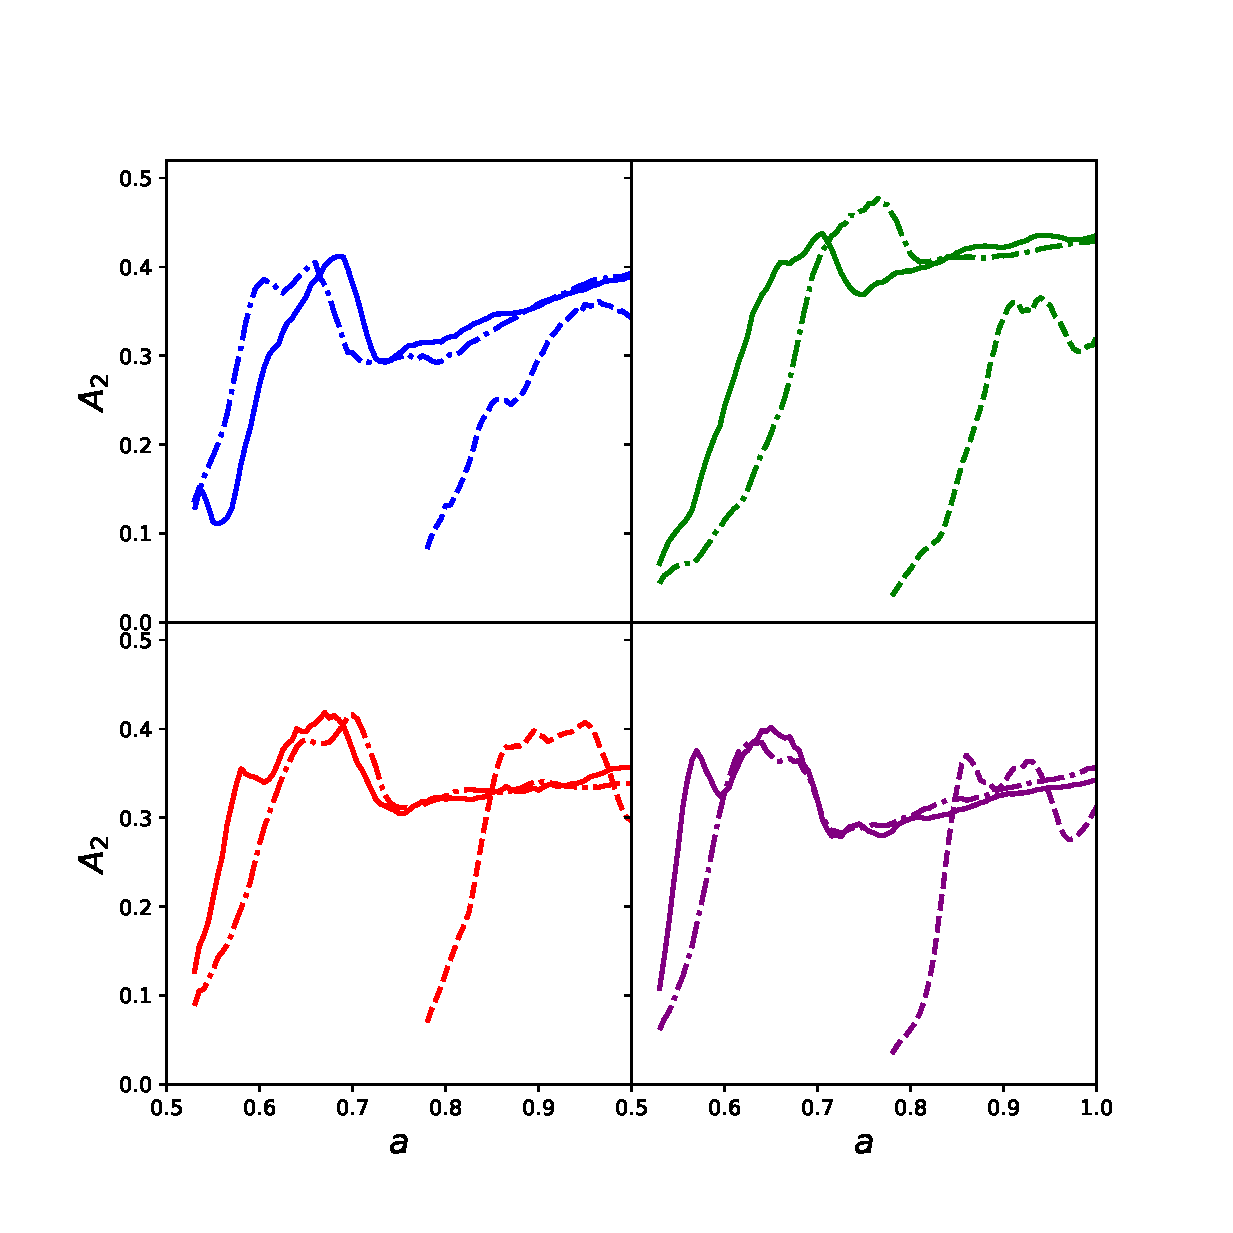
\includegraphics[width=0.85\textwidth]{../figures/a_2_all_models_four_panel.eps}
	\caption{Bar strength as measured by $A_2(<R_p)$ as a function of time for all models.} \label{fig:a_2}
\end{figure}

In isolation, a disc-halo system forms a bar when $m=2$ {density} instabilities,
seeded by shot noise-induced perturbations, exponentially grow
\citep{EfstathiouShotNoise}. Factors such as the relative contribution
of the disc to the rotation curve, radial velocity dispersion, and the
disc scale height broadly determine formation rate, strength, and
length of the bar
\citep{AthanassoulaSellwood1986,ChristodoulouStability1995,
  Klypin2009, Sellwood2013, bauer2018b}.  Strong environmental
perturbers such as halo substructure and tides can induce bar
formation even in discs that resist bar formation in isolation
\citep{gauthier_2006, kazantzidis2008, purcell2011}.

\citet{debuhr_2012,ys_2015} used a disc insertion scheme similar to
the one used here and found that in the absence of a classical bulge
stellar discs always formed bars in a cosmological environment, even
if they are submaximal.  In a previous paper, we argued that these
simulations overestimated the susceptibility of a disc to forming
strong bars \citep{bauer2018b}. This argument stems from the
observation that the discs in \citet{debuhr_2012} and \citet{ys_2015}
were too thick by a factor of $\sim 2$ as compared with the thickness
of the Milky Way and similar galaxies. We found that the more
realistic thin discs grow bars more quickly that then buckle. Since
buckling regulates the strength of the bar, the net result is that
bars in thin discs end up being weaker than those in thick discs
\citep{Klypin2009,bauer2018b}.

In Fig. \ref{fig:final_densities} we show the ratio of the surface
density across the face of the disc to the azimuthally-averaged
surface density for the final snapshots of the C.Early, C.Warm,
and C.Late simulations. Similar results are obtained for the
bauer2018, A, and B simulations. Bars form in all three simulations,
as evidenced by the X-pattern at the centre of the disc. The bar
connects with a two-armed spiral in C.Early and C.Late. The 
bar-spiral arm connection is less obvious in the C.Warm simulation.

In Fig. \ref{fig:a_2}, we plot the bar strength parameter {($\Theta=1$ in Eq. \eqref{eq:z_statistic})} evaluated in
the region $R < 2.2 R_p$ \citep{debattista_sellwood_2000}. We see that
all models experience some kind of buckling event, which reduces $A_2$
by $20-30\%$.  With the exception of bauer2018b, bar formation and
buckling is delayed in the warm disc simulations relative to the cold
disc ones.

Broadly speaking, our simulations form bars similar to that of the
Milky Way's bar in strength and length. The bulk of the bar mass in
all simulations appears contained to within $R_p = 2.2\, R_d$ The
late-insertion suite shows a reduced bar length, bolstering an idea
presented in \citet{bauer2018b} that for similar galaxies, one might
be able to use the bar length to compare relative ages of stellar
discs.

\subsection{Disc Heating}
\begin{figure}
	\centering
	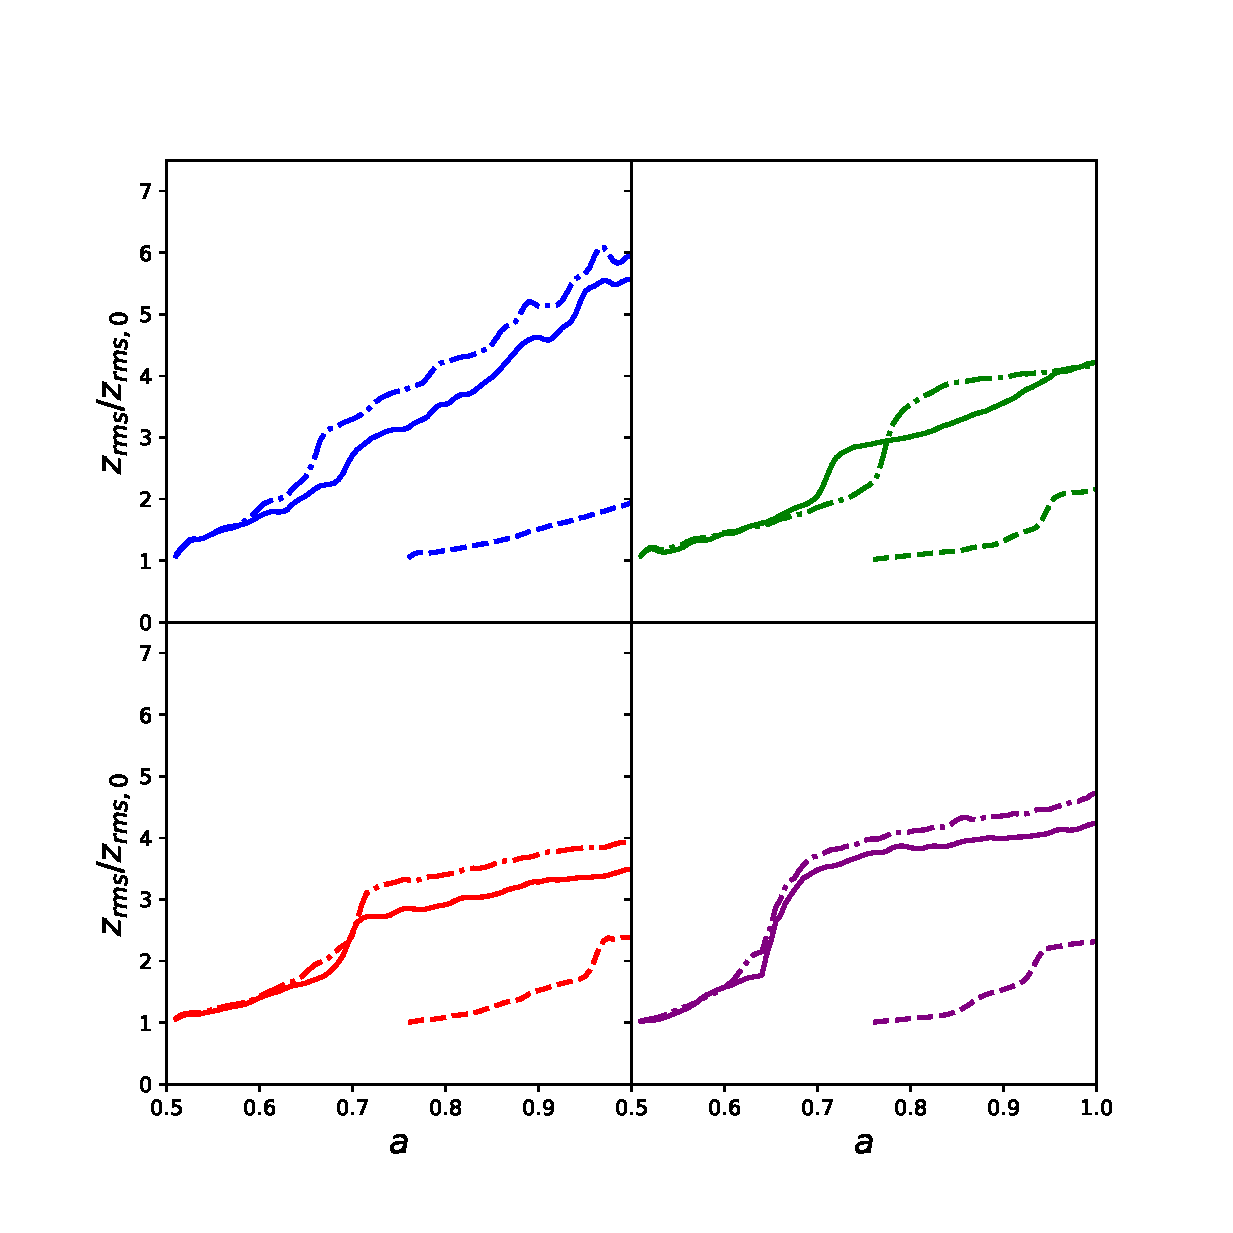
\includegraphics[width=0.85\textwidth]{../figures/z_rms_all_models_four_panel.eps}
	\caption{Disc height as measured by $z_{rms}/z_{rms,0}$ as a function of time for all models.} \label{fig:z_rms}
\end{figure}

Vertical heating and thickening in stellar discs is a well-studied
phenomenon, which can be driven by bars and spiral structure
\citep{mcmillan_dehnen_2007,Sellwood2013} or by interactions of the
disc with its satellites and its dark halo \citep[for
  example]{lacey_ostriker_1985, toth_ostriker_1992, sellwood_1998,
  bauer2018b}. These effects suggest that disc in a cosmological
environment should thicken with time, and indeed, this is confirmed in
our simulations.  Fig. \ref{fig:z_rms} shows the evolution of
$z_{rms}$ for each disc in the fiducial and warm suites. We see that
substantial heating follows bar buckling in each simulation, a result
consistent with \citet{gauthier_2006, kazantzidis2008,
  ys_2015,bauer2018b}. We note that the warm suite exhibits up to 25\%
more disc heating. There is little to say about disc heating in the
late-insertion simulations except that the discs approximately double
in thickness over the simulation time. These simulations end as the
buckling is just beginning.

\subsection{Bending waves in Cosmological Discs}

\begin{figure*}
    \centering
    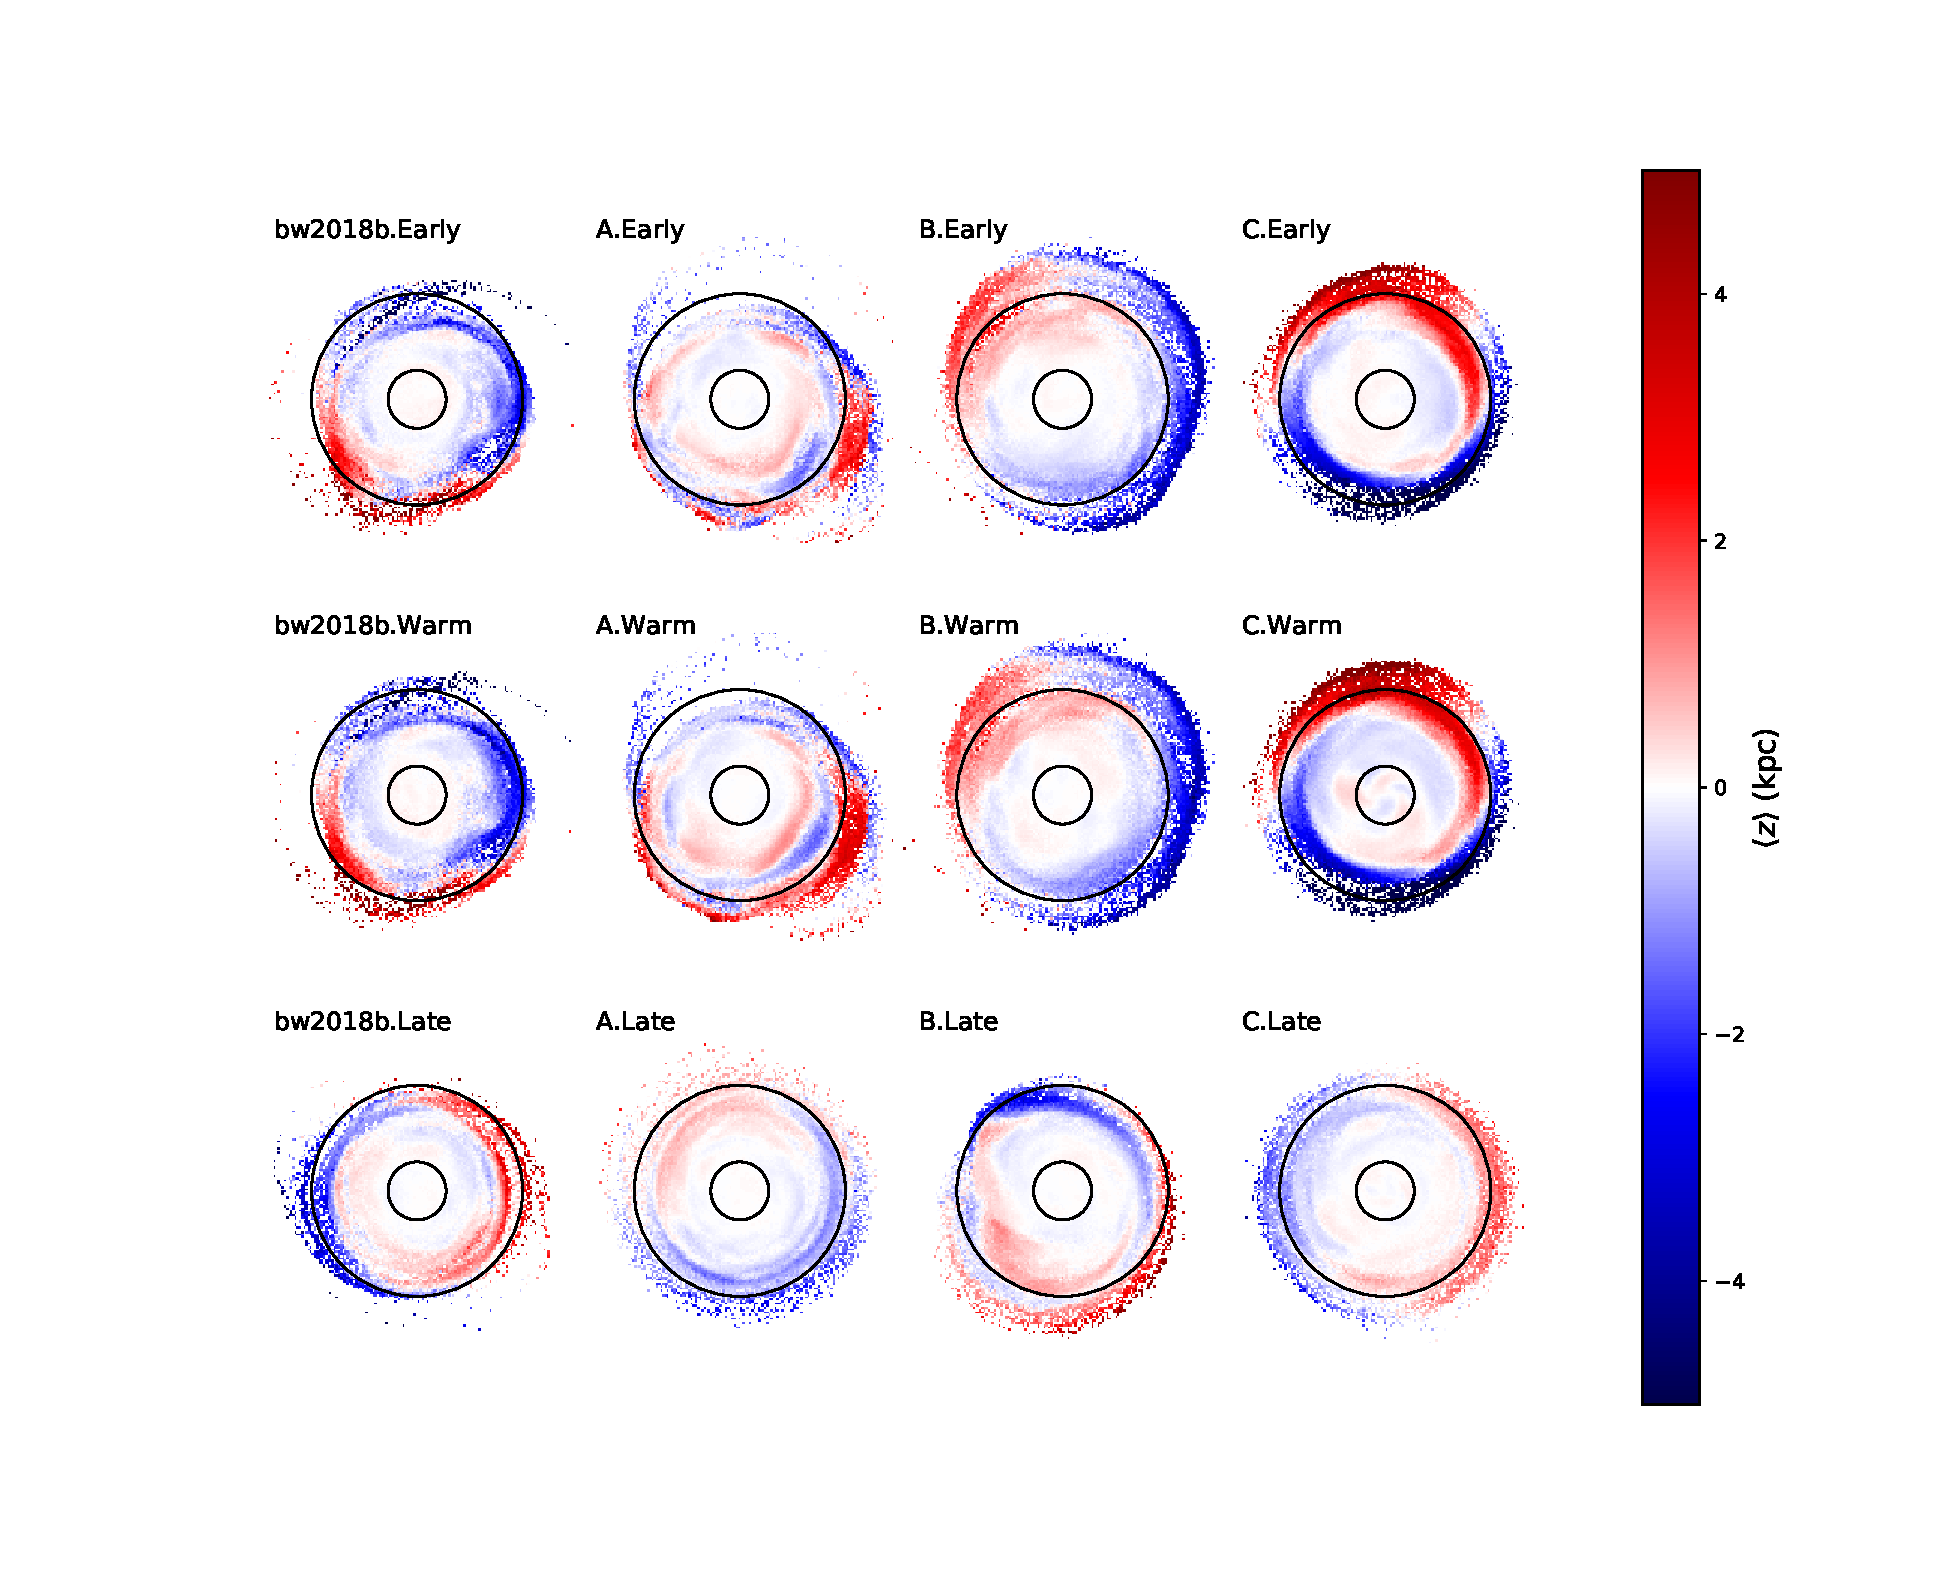
\includegraphics[width=0.9\textwidth]{../figures/twelve_panel_displacements_025.eps}
\caption{Mean displacement above or below the disc at $a=0.625$ for
  the top two rows, and $a=0.875$ for the bottom row (late-insert
  suite). The circles correspond to $2.2 \,R_d = 8.1\,\kpc$ and $20 \,
  \kpch = 29.5\,\kpc$.  }
	\label{fig:vertical_displacement_map}
\end{figure*}

\begin{figure}
	\centering
	\subfloat[]{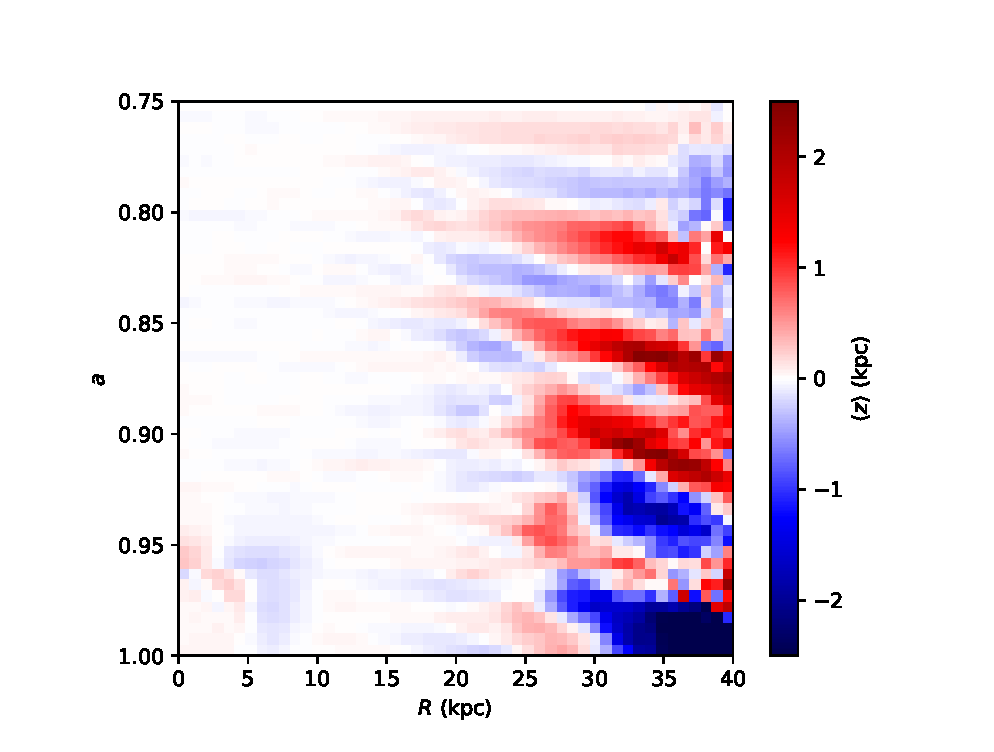
\includegraphics[width=0.45\textwidth]{../figures/b_late_z_0_r_a.eps} \label{fig:b_late_r_a}}
	\subfloat[]{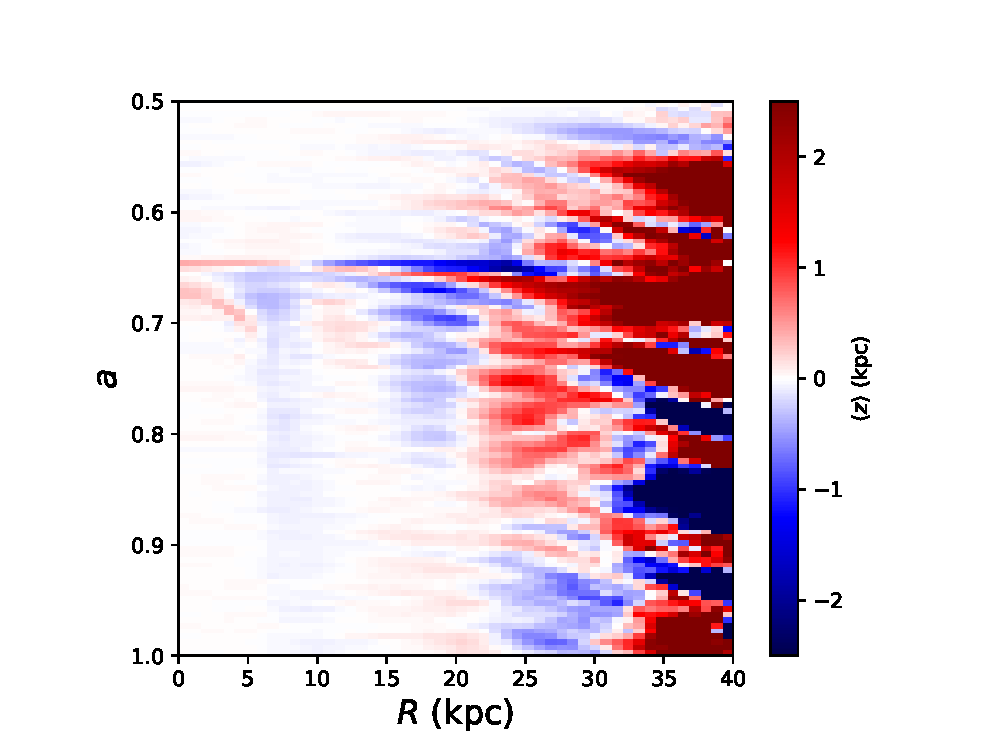
\includegraphics[width=0.45\textwidth]{../figures/c_early_z_0_r_a.eps} \label{fig:c_early_r_a}}\\
	\subfloat[]{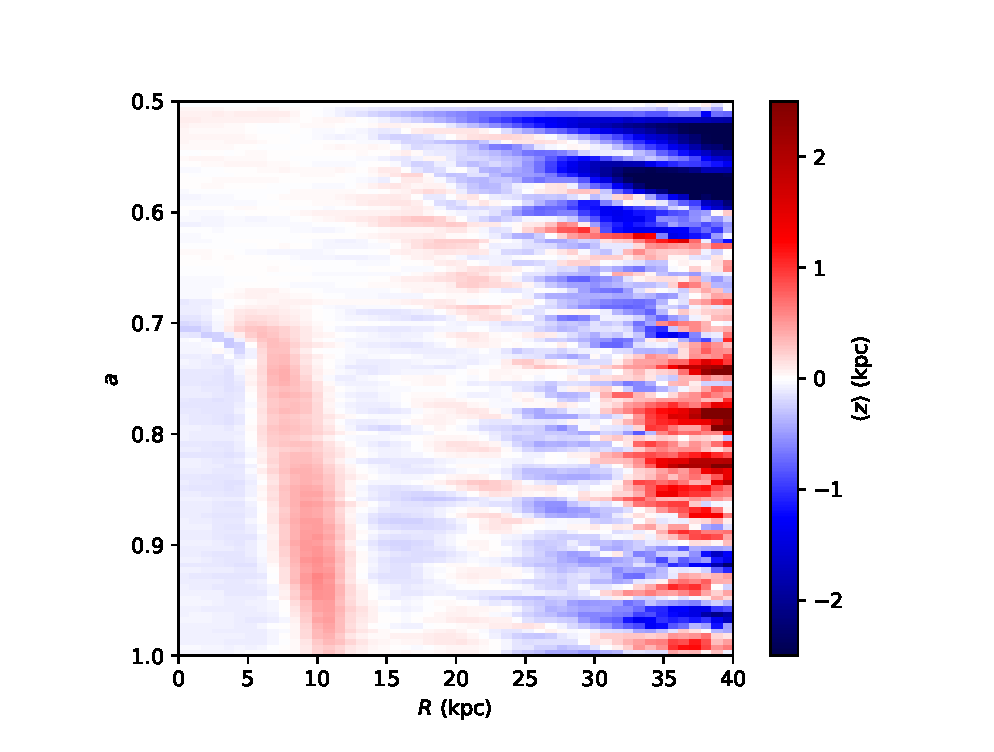
\includegraphics[width=0.45\textwidth]{../figures/a_early_z_0_r_a.eps} \label{fig:a_early_r_a}}	
\caption{The $m=0$ bending mode for B.Late (a), C.Early (b), and
  A.Early (c) as a function of radius and scale factor. }\label{fig:bendingm0}
\end{figure}

\begin{figure}
	\centering
	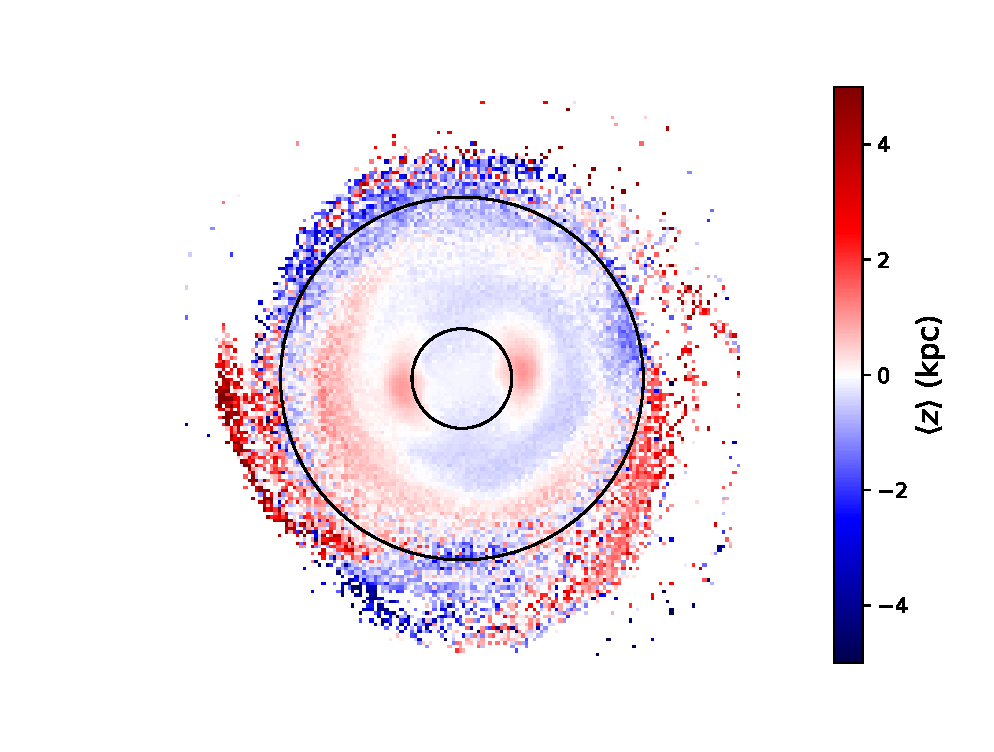
\includegraphics[width=0.85\textwidth]{../figures/a_early_displacement_a_0_875.eps}
	\caption{The mean height, $\langle z \rangle$, map for A.Early at $a=0.875$.}\label{fig:a_early_displacement}
\end{figure}

\begin{figure}\label{fig:binding_m1}
	\centering
	\subfloat[]{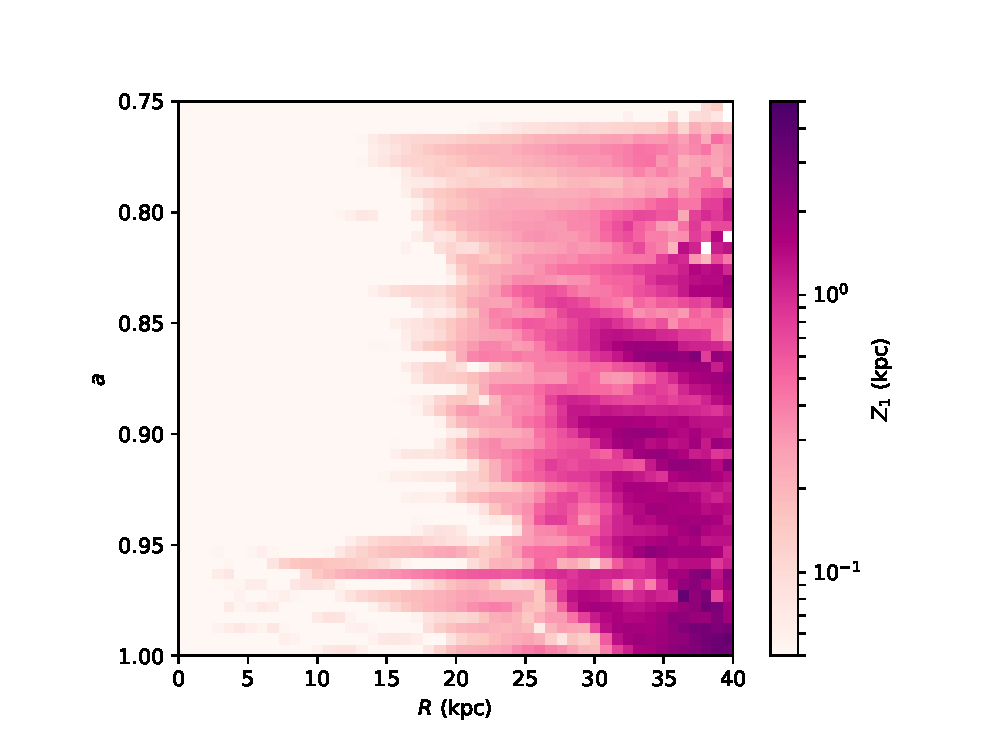
\includegraphics[width=0.45\textwidth]{../figures/b_late_z_1_r_a.eps} \label{fig:b_late_r_a_1}} \subfloat[]{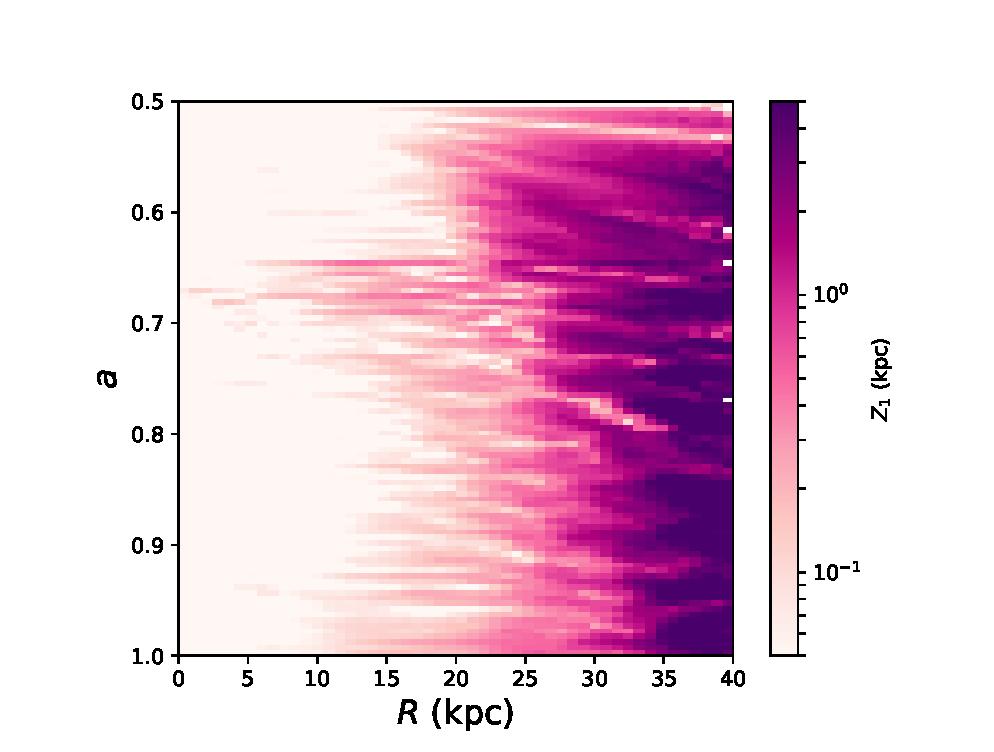
\includegraphics[width=0.45\textwidth]{../figures/c_early_z_1_r_a.eps} \label{fig:c_early_r_a_1}}\\ \subfloat[]{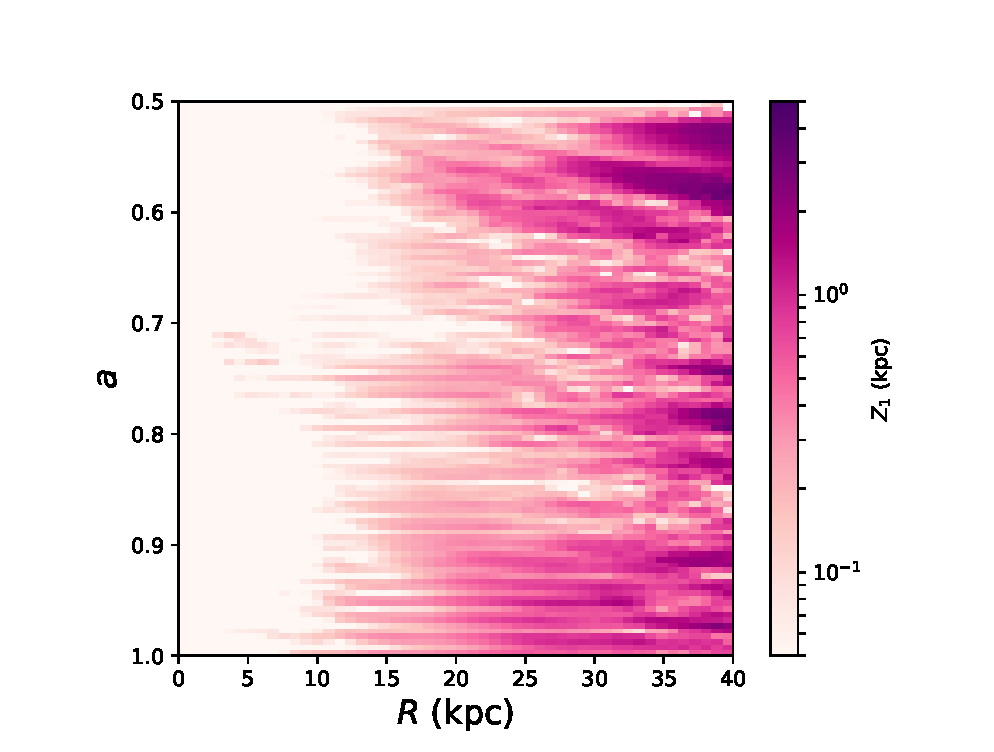
\includegraphics[width=0.45\textwidth]{../figures/a_early_z_1_r_a.eps} \label{fig:a_early_r_a_1}} \caption{The
          $m=1$ bending mode for B.Late (a), C.Early (b), and A.Early
          (c) as a function of radius and scale factor. }
\end{figure}

In Fig. \ref{fig:vertical_displacement_map} we show mean vertical
displacement ($\langle z\rangle$) maps for a single snapshot for our
twelve simulations. We choose $a=0.625$ for the early insertion runs
and $a=0.875$ for the late insertion runs. Significant warping in the
outer discs with midplane displacements of a few kiloparsecs is seen
in all simulations. However, the morphology of the warps varies
considerably. The C and bauer2018b simulations show a clear $m=1$
pattern, while the pattern in A and B is more complicated. Though the
strongest bending features are beyond $20\,{\rm kpc}$ there is clear
evidence for bending waves with amplitudes below 1 kiloparsec further
in.

In Fig.\,\ref{fig:bendingm0} we show the azimuthally-averaged ($m=0$)
bending of the disc as a function of radius and time for three of our
simulations. The B.Late simulation, where a satellite similar to the
Sgr dSph interacts with the disc shows a pattern of bending waves
similar to what we saw in the toy model presented in
\S\ref{ssec:toy_model_2} Monoceros-scale fluctuations interior to
$20\,{\rm kpc}$ occur early on and persist throughout the entire
simulation.

The evolution of $\langle z\rangle(R)$ is rather different in the
C.Early simulation, where disc-halo misalignment is driving the dynamics.
In this case, the bending waves are more like standing waves
(horizontal rather than sloping down and to the right). In addition,
there are bending waves extending all the way to the centre of the
disc, beginning when $a\simeq 0.65$. We attribute these waves the
the buckling of the bar.

Finally, we consider A.Early where the disc interacts with a
relatively massive but more distant subhalo. Bending waves set up in
the outer disc almost immediately while sub-kiloparsec corrugations
persist throughout the disc over the entire simulation. Moreover, at
$a=0.5$ a long-lived feature develops in the inner disc. To explore
this model further, we show a face-on vertical displacement map in Fig.
\ref{fig:a_early_displacement} for $a=0.875$. We interpret this feature
as a 'banana bar', that is, a bar that exibits a permanent bend along
its long axis.

In addition to flapping $m=0$ modes, we detect strong $m=1$ warp
signatures {($\Theta = z$ in Eq. \eqref{eq:z_statistic})} in our three detailed examples. In the case of the strong
satellite encounter, B.Late, we see a sub-kpc warp present in
Fig.\,\ref{fig:b_late_r_a_1} during the first half of the
simulation. As the substructure orbit continues, a close pass excites
stronger $m=1$ structures. In contrast, the strong misalignment case,
C.Early show  in Fig.\,\ref{fig:c_early_r_a_1}, exhibits kiloparsec-scale $m=1$ bending modes in the outer
disc. Furthermore, the strong $m=1$ signal extends inside of 25 kpc at
the beginning of the simulation where there is relatively little $m=0$
signature, and also where B.Late has relatively low $m=1$ signal. The
contour of the $m=1$ bending mode post-buckling roughly traces the
$m=0$ contour with a similar magnitude, suggesting a superposition of
effects brought on by the environment's coupling to the buckling
event.

The intermediate case, A.Early shown in Fig.\,\ref{fig:a_early_r_a_1}, presents something qualitatively
between B.Late and C.Early. While the outer disc is initially excited,
this behaviour subsides as the halo equilibrates. We then find
consistent, several hundred pc signal in the inner and outer disc over
the simulation. Lastly, buckling has a less drastic impact on the
$m=1$ signature for A.Early than it did for the $m=0$.

\section{KOD Dynamics} \label{sec:kud}

In this section, we focus on stars that are kick out of the disc.
We begin with a definition of a KOD star and then discuss the 
kicked-out populations in our simulations.

\subsection{Definition of a KOD star} \label{ssec:def}

\begin{figure*}
    \centering
    \subfloat[]{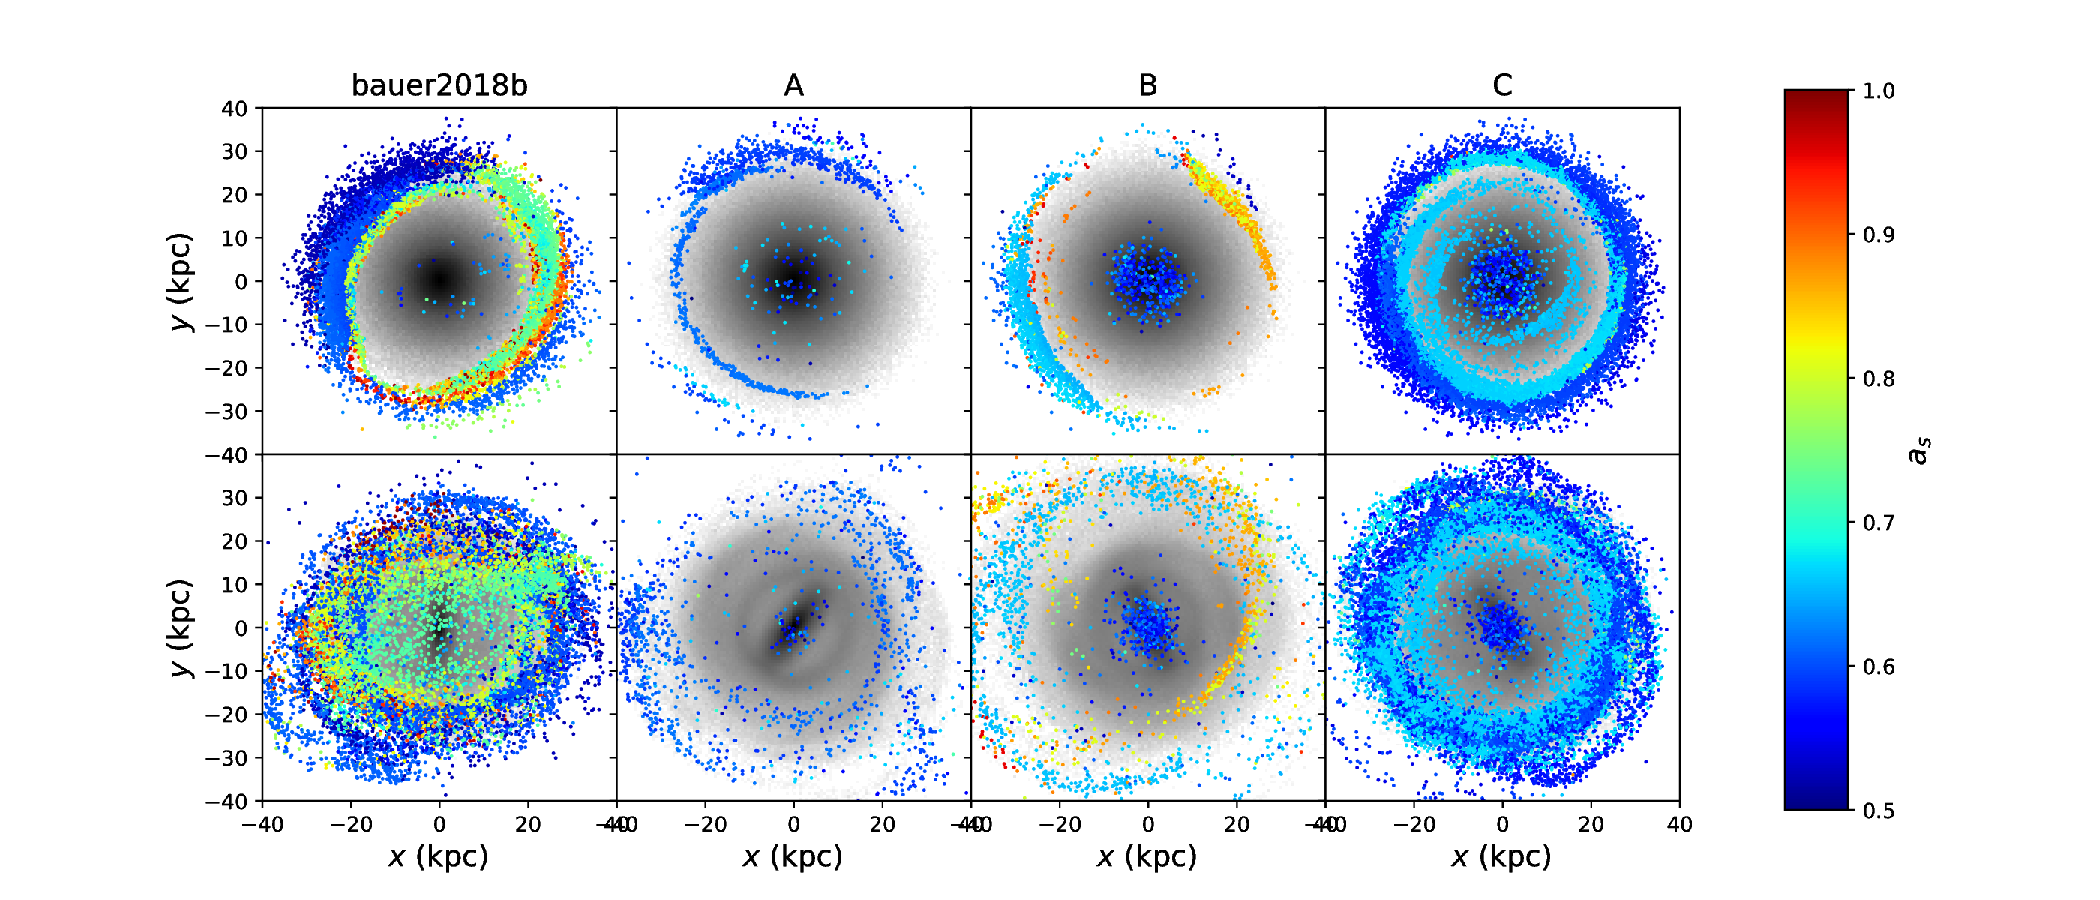
\includegraphics[width=0.9\textwidth]{../figures/kud_early_insert_face_on.pdf}}\\ 
    \subfloat[]{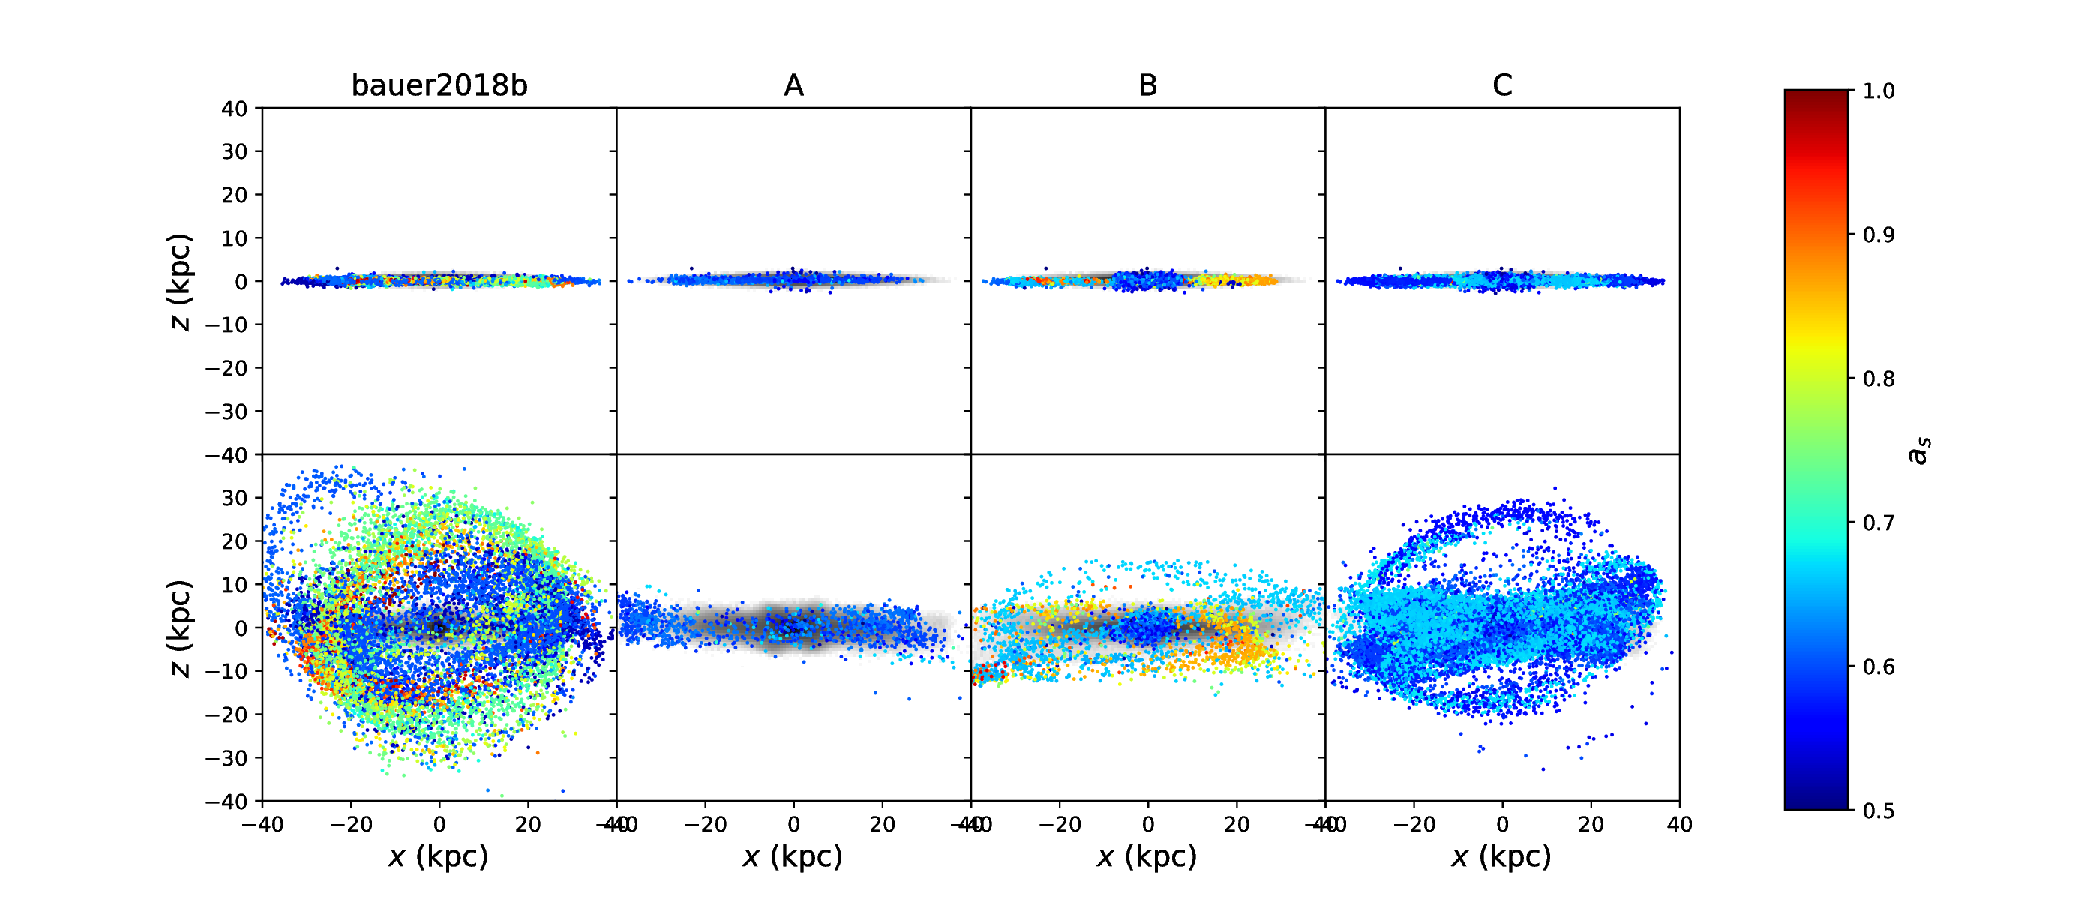
\includegraphics[width=0.9\textwidth]{../figures/kud_early_insert_edge_on.pdf}} 
\caption{KOD stars are shown for the fiducial suite in face-on (a) and
  edge-on (b) projections in the initial disc (upper panel) and final
  snapshot (lower panel). The stars not kicked out of the disc are
  shown as a histogram and the KOD stars are coloured by the time
  satisfying Eq. \ref{eq:kud_def}. Each column is one of the haloes
  considered in this paper.}
	\label{fig:kud_stars_final_ics}
\end{figure*}
We a define a kicked-out star as one where the distance from the
midplane, $|z(t)|$, exceeds some threshold, $\eta z_{\rm rms}$:
\begin{equation}
|z(t)| > \eta\,z_{\rm rms}(t)\label{eq:kud_def}
\end{equation}
where $\eta$ is a dimensionless parameter and $z_{rms}(R,\,t)$ is the
time-dependent thickness of the disc, as estimated in an annulus at
$2.2R_d$. Clearly, the choice of $\eta$ determines the number of stars
identified as being kicked out of the disc. For example,
$\eta=4$ yields 216K KOD stars or $6.2\%$ of the total stellar
content of the disc. Likewise, $\eta=8$ and $\eta=12$ yield 19K KOD
stars ($0.53\%$) and 4,302 KOD stars ($0.069\%$), respectively. These
percentages can be compared with the percentages of stars in an
exponential disc that satisfy our KOD criteria, namely
$1.8\%,\,0.034\%$, and $6\times 10^{-4}\%$, for $\eta=4,\,8,$ and
$12$, respectively. We see that for $\eta=8$ and $\eta=12$, the
number of stars identified as being kicked out exceeds the number
expected in an exponential disc by over an order of magnitude.

\begin{figure}
    \centering
    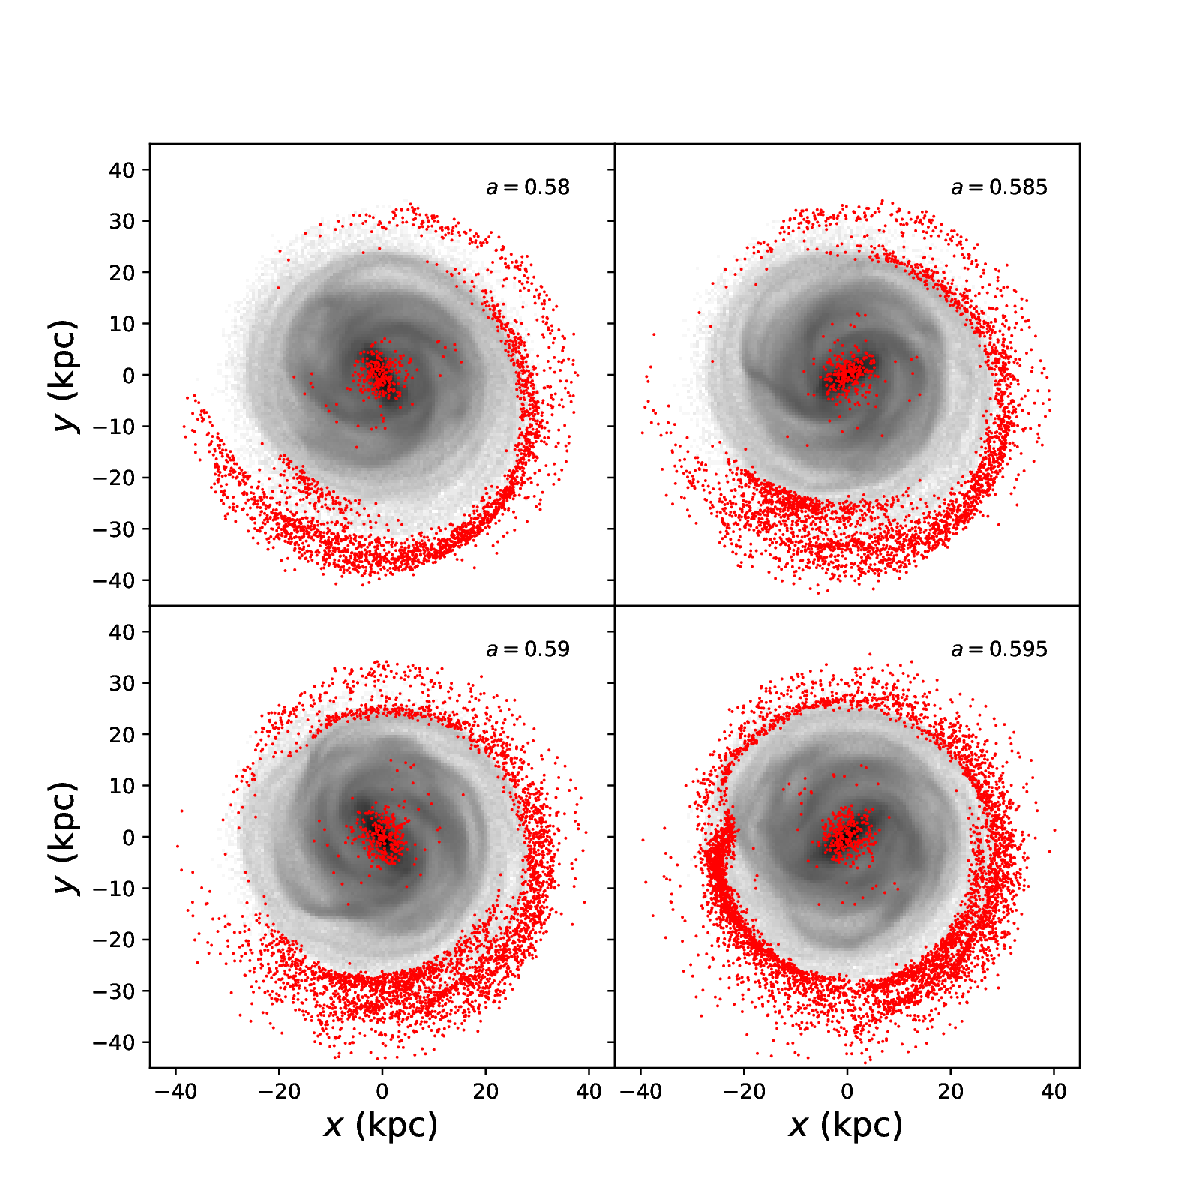
\includegraphics[width=0.85\textwidth]{../figures/fiducial_halo_268824_xy_s_016.pdf}
	\caption{KOD stars are plotted for C.Early at the labeled
          times. Note the association with spiral arms, suggesting a
          similar mechanism to \citet{laporte_2019_feathers}.}
	\label{fig:xy_tidal_tail_halo_c}
\end{figure}

\begin{figure}
    \centering
  	\subfloat[]{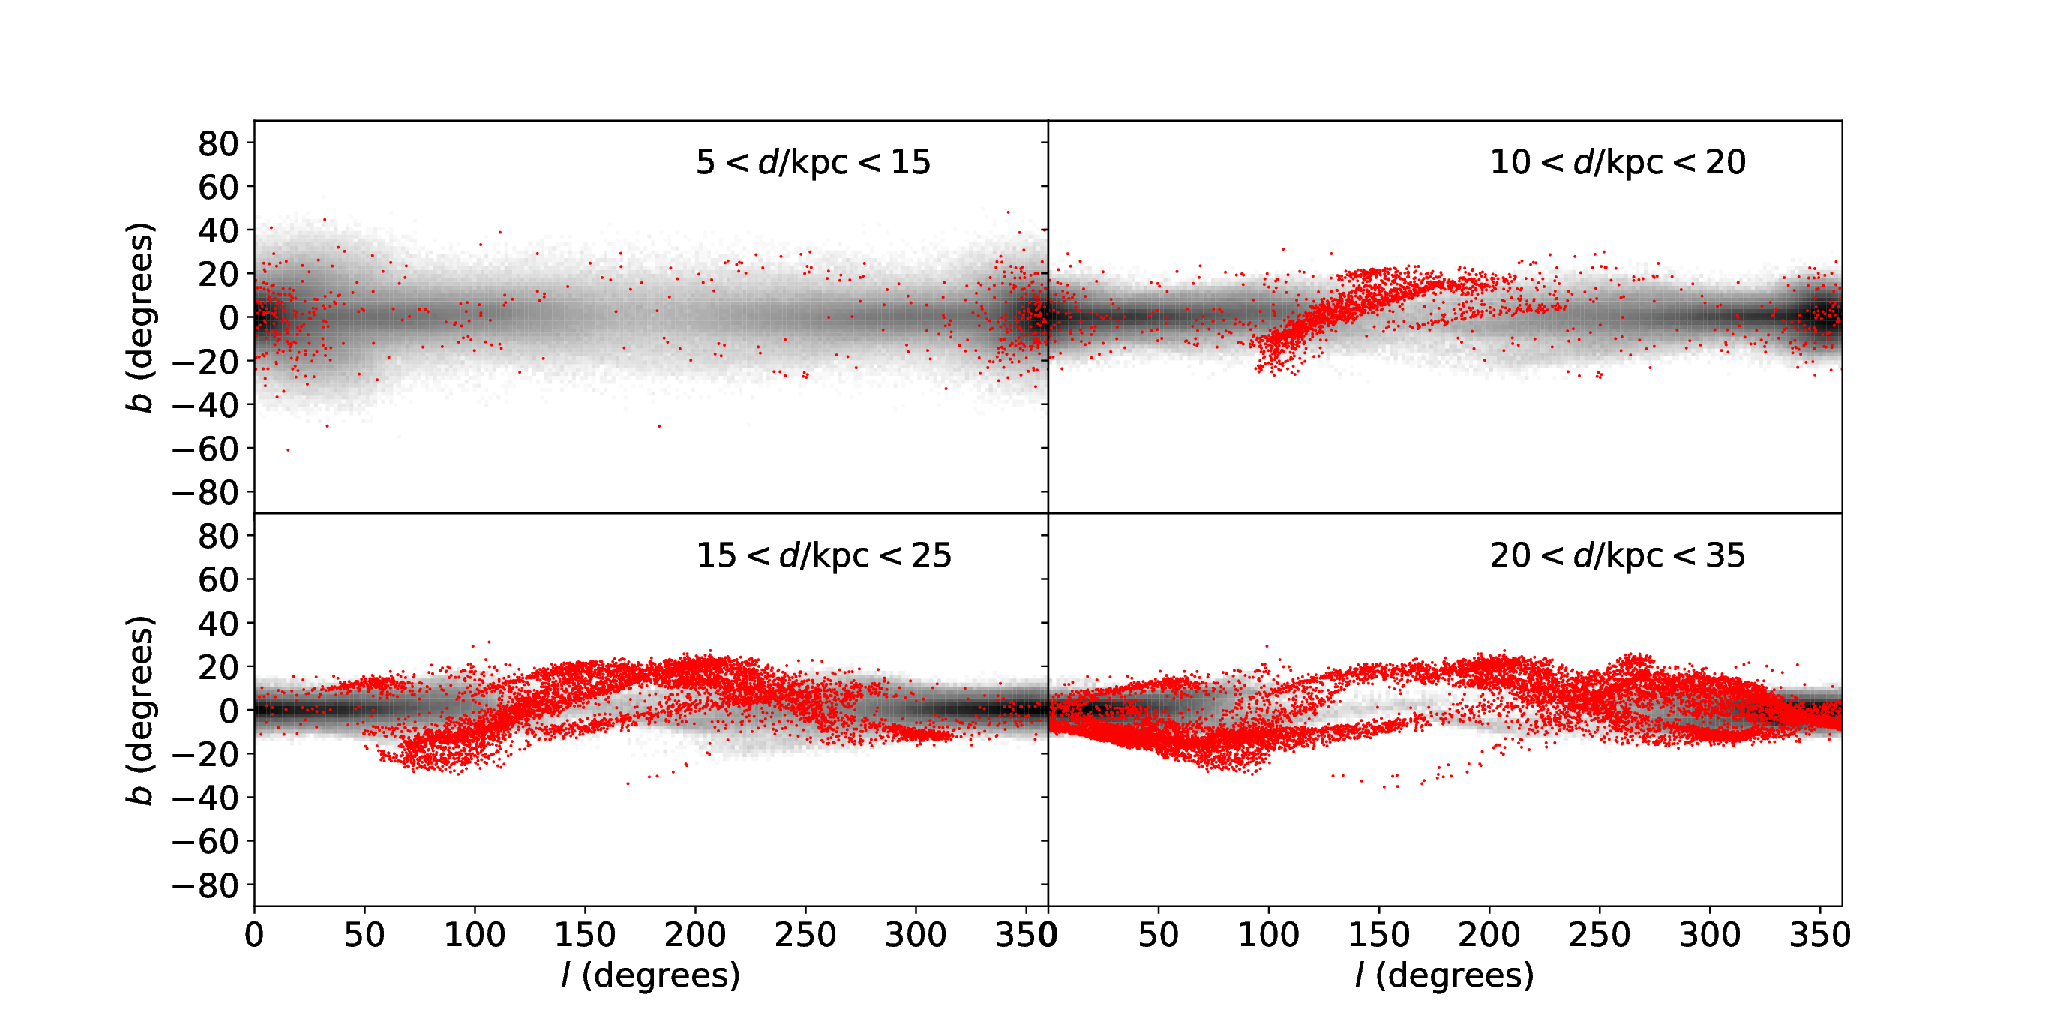
\includegraphics[width=0.85\textwidth]{../figures/fiducial_halo_268824_lb_s_055_overlay.pdf}\label{fig:lb_halo_c_warm_comparison}}\\
  	\subfloat[]{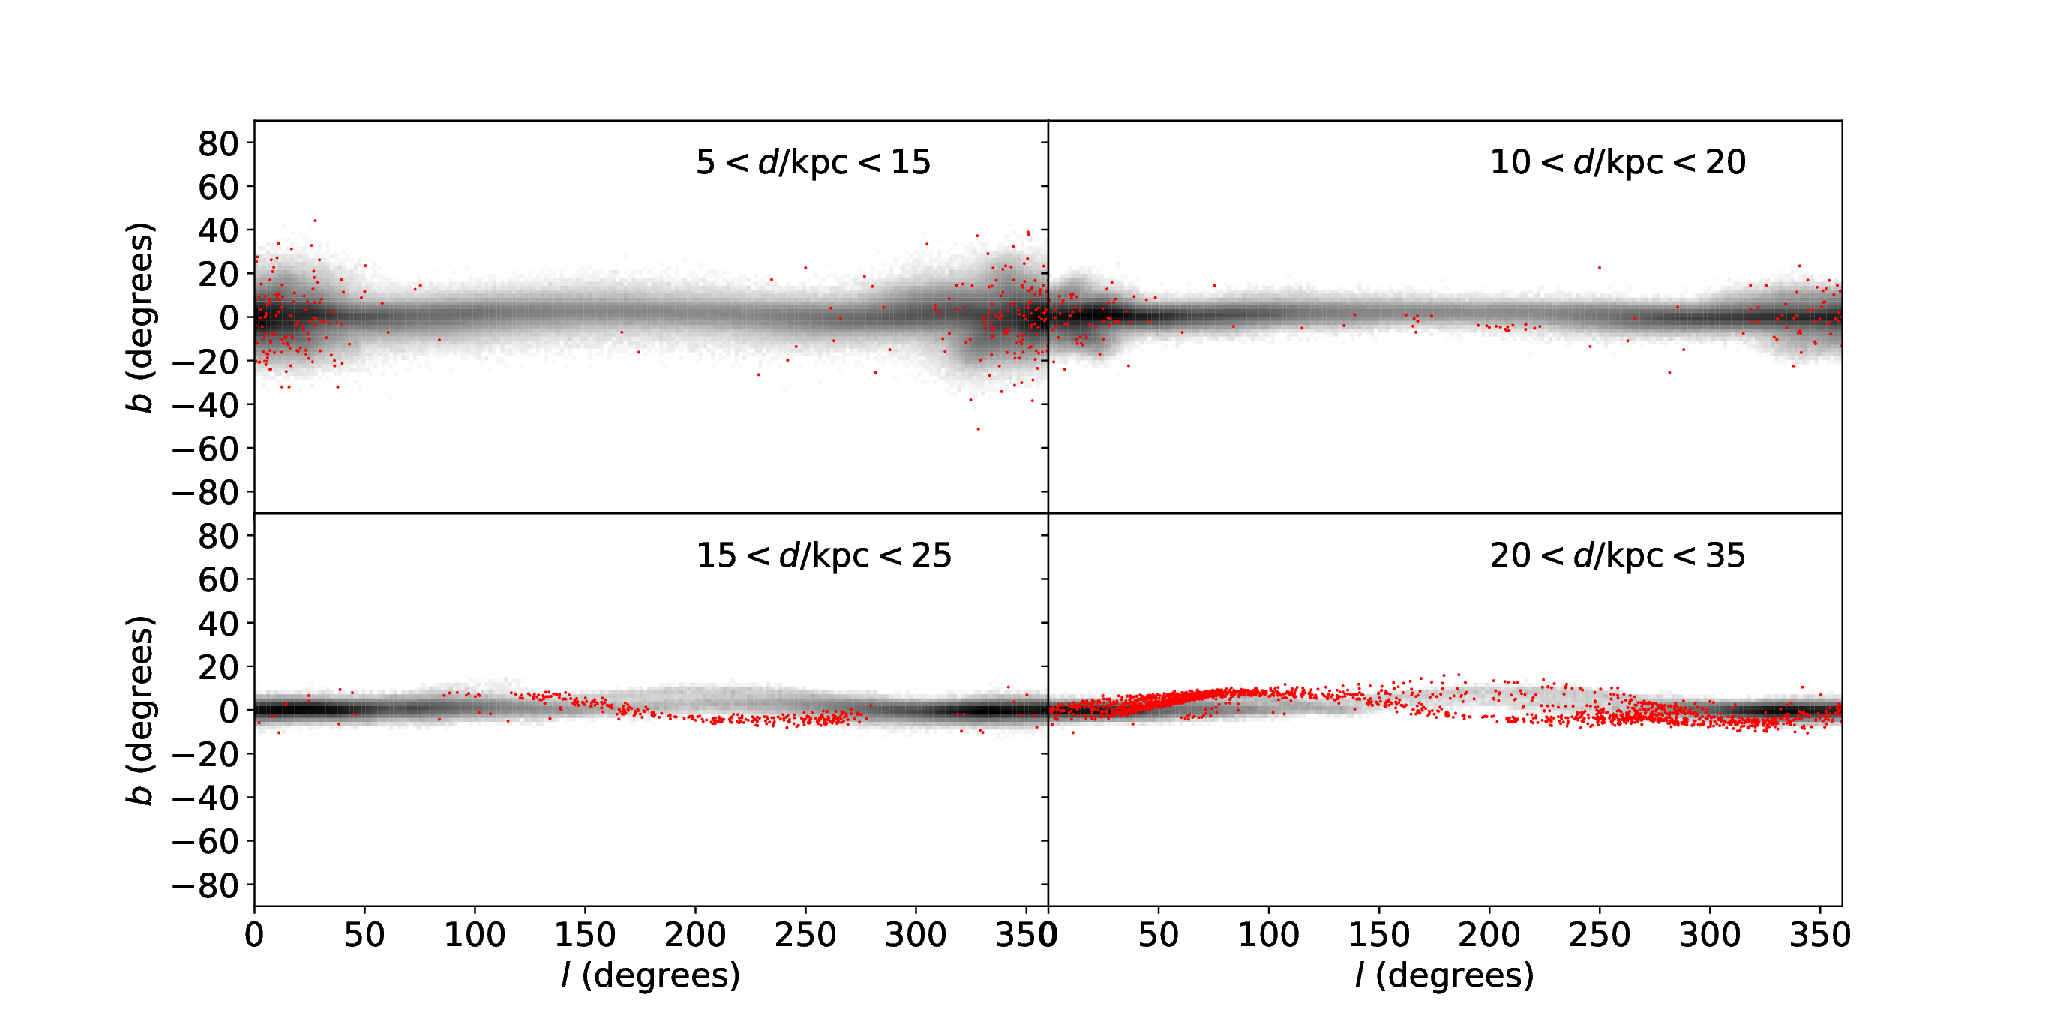
\includegraphics[width=0.85\textwidth]{../figures/fiducial_halo_268818_late_insert_lb_s_095_overlay.pdf} \label{fig:lb_halo_b_late}}
	\caption{Heliocentric views of KOD stars in several different
          distance shells. The top panel depicts this for C.Early at
          $a=0.775$. The bottom panel shows the same for B.Late at
          $a=0.975$.}
\end{figure}

\subsection{KOD Star Dynamics} \label{ssec:kud_dynamics}

We now turn our attention to the dynamics of KOD stars, identified via
Eq. \ref{eq:kud_def} with $\eta=8$ in the final
snapshot. Fig. \ref{fig:kud_stars_final_ics} shows the KOD stars in
our fiducial suite at the final snapshot. In addition, we show the
same stars traced back to their position in the initial snapshot. The
stars are color-coded by the time at which they are kicked out of the
disc.  We immediately see that the KOD structures vary markedly across
our simulations. For example, A.Early shows a relatively small KOD
population.  Moreover, the KOD structure it does have exists at very
low latitudes and was kicked out fairly early in the
simulation. B.Early has a few streams of KOD stars, which were kicked
out of the disc at roughly the time when the disc had its close
encounters with massive subhaloes. Indeed, there appear to be two
distinct populations of KOD stars. Finally, bauer2018b.Early and
C.Early show the most significant populations of KOD stars.  These
simulations correspond to the simulations with the most significant
disc-halo misalignment and shortest $T_\tau$. In both cases, we see a
continuous range of times over which stars were kicked out. Moreover,
in C.Early, many of the KOD stars were originally in the inner disc.

The mechanism in C.Early by which stars from the inner disc can be
kicked out is highlighted in Fig. \ref{fig:xy_tidal_tail_halo_c}. Each
new round of KOD stars appears to be associated with a spiral pattern
of small pitch angle. Together with
Fig. \ref{fig:kud_stars_final_ics}, we are left with the picture that
KOD stars generally originate in the outer disc though in some cases,
such as C.Early, strong spiral structure transfers stars outward and
into strong warps. Stars in these warps can then be easily stripped
from the disc. The stripped stars in turn phase mix to form the
high-latitude structures seen in the final snapshot of C.Early.  Stars
associated with the features seen in
Fig. \ref{fig:xy_tidal_tail_halo_c} form filamentary structures with a
characteristic bifurcation, which \citet{laporte_2019_feathers}
referred to as ``feathers".

In Fig. \ref{fig:lb_halo_c_warm_comparison}, we see the KOD stars in
C.Early as they appear from the Solar neighborhood at $a=0.775$. The
stars form the top and bottom feather structure described in
\citet{laporte_2019_feathers}, and are undoubtedly associated with
grand design spiral structure. The similarities suggest that
large-scale tidal fields create observable, stream-like structures at
low-to-mid Galactic latitudes, extending along the length of the sky.
We contrast this with B.Late, where there is a moderate-mass
($10^{10}\,M_\odot$) Sgr interaction. From the perspective of the Sun,
KOD structures present in B.Late and shown in
Fig. \ref{fig:lb_halo_b_late} appear at relatively low latitudes. Thus
a moderate-mass Sgr dSph does not appear to be capable of exciting
high latitude structures on a short timescale.

\section{Discussion} \label{sec:discussion}

\subsection{Disc Flapping}

Perhaps the most novel effect that we have explored is the generation
of flapping modes from differential acceleration of the disc by
distant subhaloes and other mass concentrations in a $\Lambda$CDM cosmology.
\citet{sellwood_1996} presented the first in-depth study
of this phenomenon in isolated galaxies. We find that the disc
flapping naturally arises in the cosmological environment and can be
due to one of three mechanisms: two-body interaction of the 
disc and inner halo with a subhalo, buckling of the bar,
and torquing of the disc by its smooth, triaxial halo.

There is reason to think that the first of these mechanisms is is
secondary to the others. \citet{gomez_2017} ran MHD simulations
where they note a lack of U-shaped ($m=0$) warps, which would
presumably be caused by flapping. Conversely, they found that S-shaped
($m=1$) warps were fairly common. In our suite of simulations, B.Late
provides the best example where flapping modes from a distant subhalo can be seen as the
dominant effect; it has no buckling bar and is initialized in a quiet
halo. For both A.Early and C.Early, we would be hard pressed to say
that we see the same kind of behaviour, especially where the disc is
decently resolved.

The bar buckling generation mechanism for flapping modes is
prominently displayed in C.Early. After the bar buckles, we see
axisymmetric fluctuations in the mean height, as well as substantial
flapping in the region of Monoceros. C.Early is clearly an outlier in
this respect, and we suggest that bar buckling in conjunction with
triaxility is a viable mechanism for corrugations in cosmological
simulations. The general effect of bar buckling appears to introduce a
signal in mean height, consistent with the simulation in
\citet{bar_buckling_echo}.

\subsection{Bending waves, KOD stars and feathers}

Consistent with \citet{gomez_2017}, we find that halo misalignment is
not a likely source of bending in the inner disc. Rather, most of the
$m=0$ and $m=1$ waves in the inner disc appear to be associated with
bar buckling. However, the outer disc is most definitely affected by
the smooth halo's tides. We see this in C.Early's $m=1$ profile, which
is much stronger than that in either B.Late or A.Early.

\citet{laporte_2018_b} and \citet{laporte_2019_feathers} found that a
massive Sgr-like dwarf ($M \simeq 8 \times 10^{10} \, \solarm$ and
above) whose orbit passes through the Galactic midplane several times
can produce populations of KOD stars consistent with those observed
in the Milky Way. It is worth noting that their proposed mass is at
the higher end of estimates for the mass of the Sgr dSph
progenitor, and twice the mass of the stellar disc in our simulations. Our B.Late simulation provides an example of an encounter
with a $3 \times 10^{10}$ subhalo that passes through the disc plane
at $a=0.875$ on an orbit that is similar to model L1 in
\citet{laporte_2018_b}. Consistent with their findings, it appears
that even this quite massive perturber cannot excite the requisite
structures. On the other hand, we do find KOD stars in other
simulations within our suite where the main disc-environment effects
come from large-scale tidal fields. Indeed, the simulations in which
KOD stars reach their highest latitudes are the ones with substantial
inner-halo-disc axis misalignment, namely C.Early and
bauer2018b.Early. These are also the simulations with the highest
$m=1$ bending signature in the outer disc.  Thus, kicking stars to
higher latitudes either requires an extremely massive perturber or
substantial misalignment with the host halo.

Our results are consistent with those of \citet{laporte_2019_feathers}
who found that KOD stars remain close to each other in phase space. For
instance, in B.Late stars are kicked out of the disc at two discrete
times from narrow regions of the disc. By the end of the simulation,
these stars are still closely associated with each other.  We can also
infer from our simulations that for some mono-abundant chemical
population at $z=1$, we would expect to see dynamically coherent (as
supported by how stars are clustered by their kick-up time in the
final snapshot) structures with a consistent chemical abundance. This
result is consistent with observations by \citet{bergemann_2018}, who
found narrow abundance spreads for M-giants in A13 and TriAnd. The
clustering of stars by their kickup time is true whether they were
kicked by substructure, as in B.Late, or by the smooth halo, as in
C.Early.

\section{Conclusions}\label{sec:conclusion}
{We have presented a suite of simulations in which stellar discs are
inserted into cosmological haloes. These haloes are, in general,
triaxial and clumpy and drive the disc from its initial axisymmetric
and near equilibrium state to one of disequilibrium. The key findings are summarized as:
\begin{itemize}
\item All discs all form bars, even though buckling can regulate their strengths.
\item All discs exhibit some kind of bending and warping.
\item Disc flapping is a major manifestation of disequilibrium in the cosmological environment.
\item Subhaloes with a mass lower than that of the disc are unlikely to generate KOD populations.
\end{itemize}}
{It is not surprising that} the discs in our simulations bend and warp. In
addition, we find large populations of stars kicked out of the disc.
These departures from planarity signal a state of disequilibrium {likely present in the Milky Way}.  We
have identified several mechanisms for generating vertical structure, which
include the well-studied interaction of the disc with a massive
satellite, differential acceleration of the disc due to tidal fields
of the halo or a distant massive satellite, and the buckling bar.
The first two mechanisms can produce large warps (amplitudes of
order 1-3 kpc) in the outer disc along with smaller amplitude 
waves that extend further in. On the other hand, the buckling bar
is efficient at producing bending waves and corrugation patterns 
in the inner disc.

{Absent substantial global tides, the KOD populations we see are not able to reach high latitudes. As such, o}ur findings are consistent with the idea that a subhalo less
massive than the disc is unlikely to be responsible for even low
latitude streams seen in the Milky Way. On the other hand, disc-halo
misalignment can generate these populations quite easily. {Taken in whole, our analysis suggests that studies which focus on only one mechanism of vertical structure generation are unlikely to capture the full picture. We have done out best to disentangle the different mechanism of disequilibrium. Future work will attempt to determine which ones dominate in the Milky Way.}

\section*{Acknowledgements}
{LMW and JSB are supported by a Discovery Grant with the Natural
  Sciences and Engineering Research Council of Canada.}
  
  
\bibliographystyle{apalike}
\bibliography{bibliography_paper_iii.bib} % if your bibtex file is called example.bib


%%%%%%%%%%%%%%%%%%%%%%%%%%%%%%%%%%%%%%%%%%%%%%%%%%


